%!TEX root=./LIVRO.tex
\pagebreak
%\pagestyle{simu}
\addcontentsline{toc}{chapter}{SIMULADO 1}
\markboth{Simulado 1}{}

\num{1} NO PACOTE DE AÇÚCAR QUE COMPRAMOS NO SUPERMERCADO, GERALMENTE HÁ UM NÚMERO
1 SEGUIDO DA UNIDADE ``KG''. O QUE ESSE NÚMERO REPRESENTA?

\begin{escolha}
\item CÓDIGO DE IDENTIFICAÇÃO.

\item MEDIDA.

\item QUANTIDADE.

\item ORDEM.
\end{escolha}

\num{2} ANALISE O ALFABETO.

%\textless{}https://br.freepik.com/vetores-gratis/fontes-alfabeto-inglesas-em-cores-diferentes\_1372652.htm\#query=alfabeto\&position=1\&from\_view=search\&track=sph\textgreater{}

\begin{figure}[H]
\centering
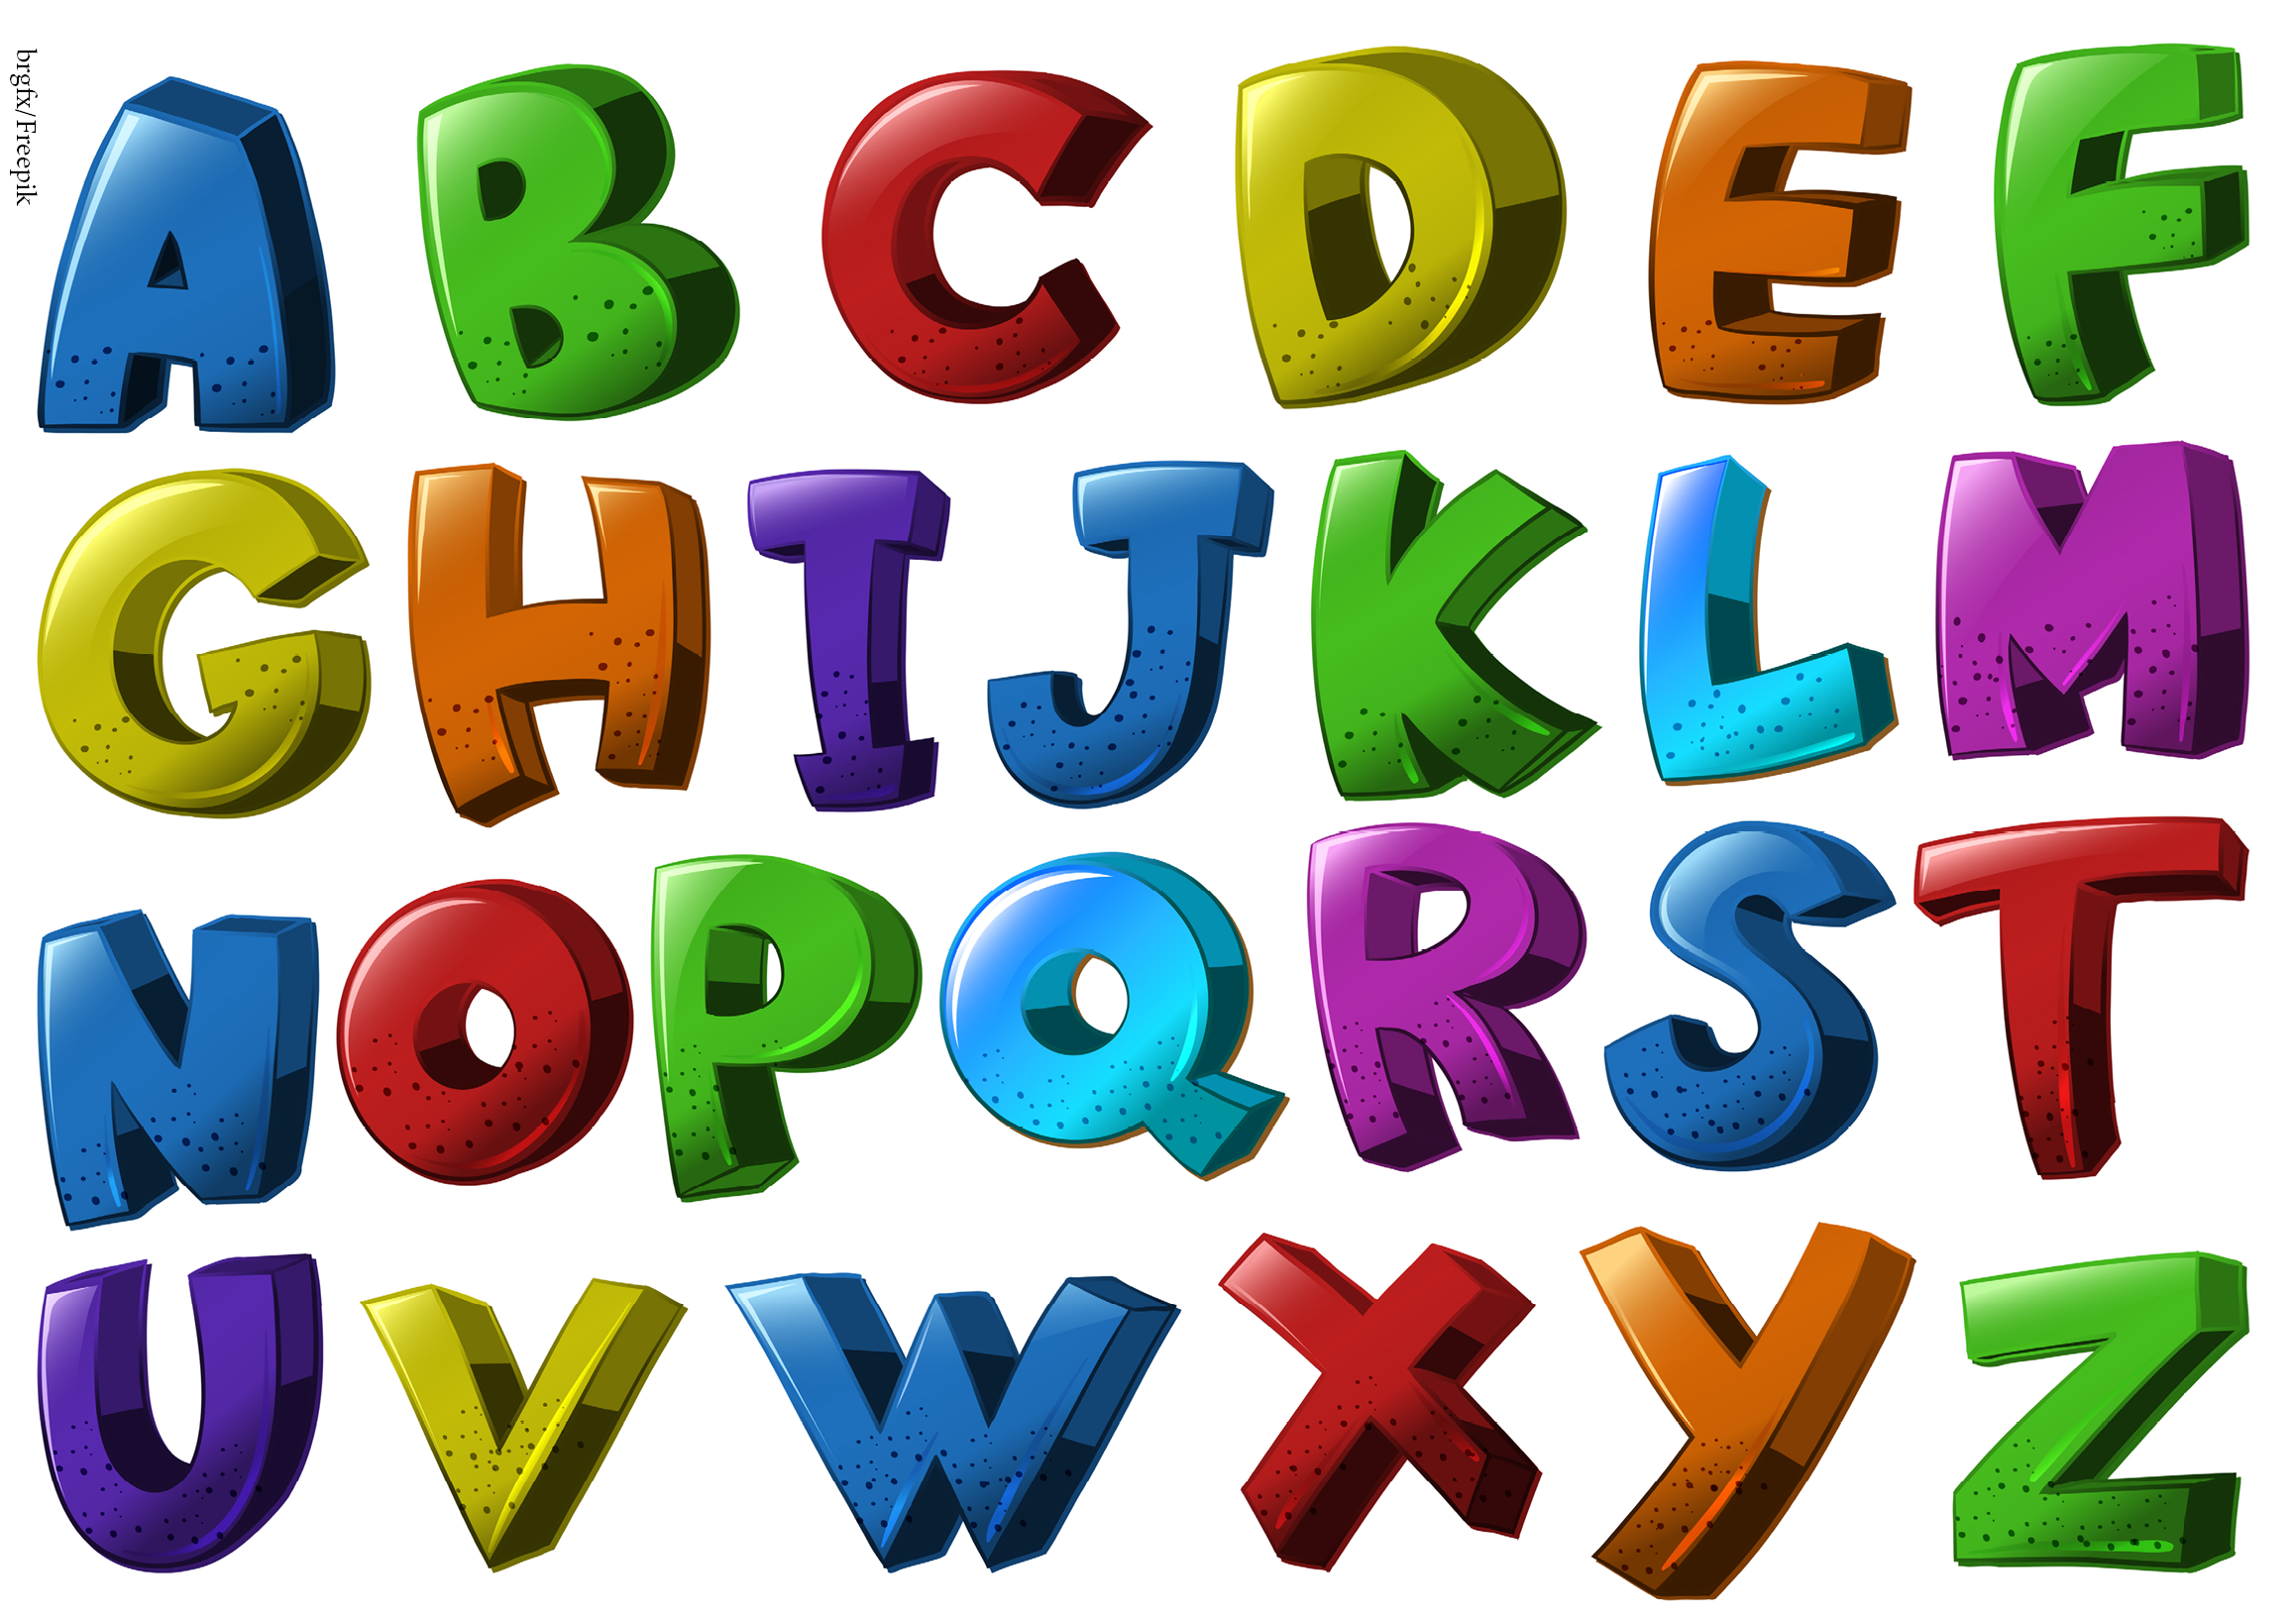
\includegraphics[width=.8\textwidth]{./media/SAEB_1ANO_MAT_FIGURA112.png}
\end{figure}

INDIQUE QUAL É A POSIÇÃO DA LETRA G.

\begin{escolha}
\item 5 (QUINTA LETRA).

\item 6 (SEXTA LETRA).

\item 7 (SÉTIMA LETRA).

\item 8 (OITAVA LETRA).
\end{escolha}


\num{3} OBSERVE A SOMA.\bigskip

\hspace*{\fill}\adjustbox{varwidth=.5\linewidth}{
\begin{mdframed}[linewidth=2pt,linecolor=salmao,backgroundcolor=salmao!20,roundcorner=10pt]
\centering\LARGE
64 + 46
\end{mdframed}
}\hspace*{\fill}

\vspace{1cm}

O RESULTADO É

\begin{escolha}[itemsep=0pt]
\item 18.

\item 100.

\item 101.

\item 110.
\end{escolha}

\num{4} INDIQUE UMA FORMA CORRETA DE COMPOR O NÚMERO 50.

\begin{escolha}[itemsep=0pt]
\item 25 + 26.

\item 35 + 25.

\item 98 -- 48.

\item 100 -- 45.
\end{escolha}

\num{5} ANALISE A IMAGEM.

%\textless{}Criar uma figura com dois lápis, conforme o modelo a seguir. Utilize a referência: https://br.freepik.com/vetores-premium/icone-de-lapis-em-estilo-simples-ilustracao-vetorial-de-equipamentos-de-educacao-em-fundo-isolado-conceito-de-negocio-de-sinal-de-ferramenta-de-desenho\_30026502.htm\#query=lapis\&position=6\&from\_view=search\&track=sph.\textgreater{}

\begin{figure}[H]
\centering

\includegraphics[width=.5\textwidth]{./media/SAEB_1ANO_MAT_FIGURA113.png}
\end{figure}

SOBRE OS DOIS LÁPIS DA IMAGEM, PODE-SE DIZER QUE

\begin{escolha}[itemsep=0pt]
\item ELES TÊM O MESMO COMPRIMENTO.

\item O LÁPIS DE BAIXO TEM MENOR COMPRIMENTO.

\item O LÁPIS DE CIMA TEM MENOR COMPRIMENTO.

\item OS COMPRIMENTOS DELES NÃO PODEM SER COMPARADOS.
\end{escolha}

\num{6} OBSERVE A IMAGEM.

%\textless{} https://br.freepik.com/vetores-gratis/adesivo-de-copo-de-medicao-em-fundo-branco\_18180135.htm\#query=COPO\%20MEDIDORDESENHO\&position=2\&from\_view=search\&track=ais. Colocar as quantidades conforme o modelo a seguir.\textgreater{}

\begin{figure}[H]
\centering

\includegraphics[width=.3\textwidth]{media/image107.jpg}
\end{figure}

QUE TIPO DE MEDIDA É CONSEGUIDO PELO INSTRUMENTO REPRESENTADO?

\begin{escolha}[itemsep=-5pt]
\item CAPACIDADE.

\item COMPRIMENTO.

\item MASSA.

\item TAMANHO.
\end{escolha}

\num{7} OBSERVE A CONFUSA E DESORDENADA LISTA DE TAREFAS DE CARLOS PARA UM DIA
QUALQUER.

% \begin{figure}[htpb!]
% \centering
% 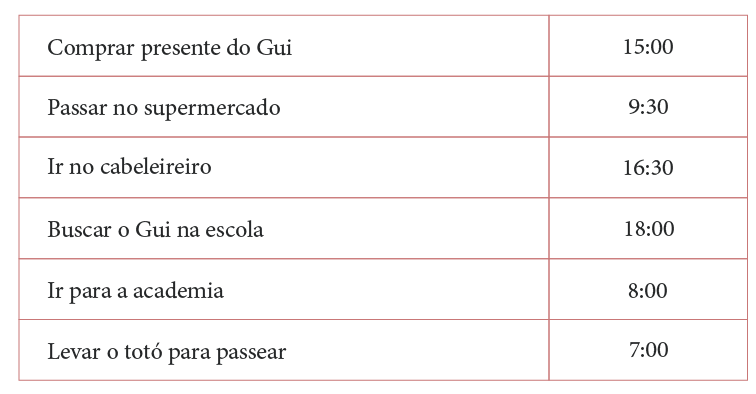
\includegraphics[width=.6\textwidth]{./media/SAEB_1ANO_MAT_FIGURA115.png}
% \end{figure}

\begin{myquote}
\begin{itemize}
  \item \textbf{15:00} --- \uppercase{Comprar o presente do Gui.}
  \item \textbf{9:30} --- \uppercase{Passar no supermercado.}
  \item \textbf{16:30} --- \uppercase{Ir ao cabeleireiro.}
  \item \textbf{18:00} --- \uppercase{Buscar o Gui na escola.}
  \item \textbf{8:00} --- \uppercase{Ir para a academia.}
  \item \textbf{7:00} --- \uppercase{Levar o cachorro para passear.}
\end{itemize}
\end{myquote}

QUAL É A TERCEIRA ATIVIDADE DE CARLOS DURANTE ESSE DIA?

\begin{escolha}[itemsep=-5pt]
\item BUSCAR O GUI NA ESCOLA.

\item COMPRAR O PRESENTE DO GUI.

\item LEVAR O CACHORRO PARA PASSEAR.

\item PASSAR NO SUPERMERCADO.
\end{escolha}

\num{8} OBSERVE O CALENDÁRIO A SEGUIR.\bigskip

\begin{table}[H]\footnotesize
\centering
\begin{tabular}{|ccccccc|}
\hline
\multicolumn{7}{|c|}{FEVEREIRO/2023} \\ \hline
\multicolumn{1}{|c|}{DOM} & \multicolumn{1}{c|}{2ª FEIRA} & \multicolumn{1}{c|}{3ª FEIRA} & \multicolumn{1}{c|}{4ª FEIRA} & \multicolumn{1}{c|}{5ª FEIRA} & \multicolumn{1}{c|}{6ª FEIRA} & SÁBADO \\ \hline
\multicolumn{1}{|c|}{} & \multicolumn{1}{c|}{} & \multicolumn{1}{c|}{} & \multicolumn{1}{c|}{1} & \multicolumn{1}{c|}{2} & \multicolumn{1}{c|}{3} & 4 \\ \hline
\multicolumn{1}{|c|}{5} & \multicolumn{1}{c|}{6} & \multicolumn{1}{c|}{7} & \multicolumn{1}{c|}{8} & \multicolumn{1}{c|}{9} & \multicolumn{1}{c|}{10} & 11 \\ \hline
\multicolumn{1}{|c|}{12} & \multicolumn{1}{c|}{13} & \multicolumn{1}{c|}{14} & \multicolumn{1}{c|}{15} & \multicolumn{1}{c|}{16} & \multicolumn{1}{c|}{17} & 18 \\ \hline
\multicolumn{1}{|c|}{19} & \multicolumn{1}{c|}{20} & \multicolumn{1}{c|}{\textcolor{blue}{21}} & \multicolumn{1}{c|}{22} & \multicolumn{1}{c|}{23} & \multicolumn{1}{c|}{24} & 25 \\ \hline
\multicolumn{1}{|c|}{26} & \multicolumn{1}{c|}{27} & \multicolumn{1}{c|}{28} & \multicolumn{4}{l|}{\textcolor{blue}{21 -- CARNAVAL}} \\ \hline
\end{tabular}\bigskip
\end{table}

INDIQUE EM QUE DIA DA SEMANA CAIU O CARNAVAL.

\begin{escolha}
\item SÁBADO.

\item DOMINGO.

\item SEGUNDA-FEIRA.

\item TERÇA-FEIRA.
\end{escolha}

\num{9} OBSERVE AS IMAGENS.

%\textless{} https://www.istockphoto.com/br/foto/brasileiro-dinheiro-novo-gm492403659-40519468?phrase=5\%20REAIS; https://www.istockphoto.com/br/foto/brasileiro-dinheiro-novo-gm492403657-40519264.\textgreater{}

\begin{figure}[H]
\centering
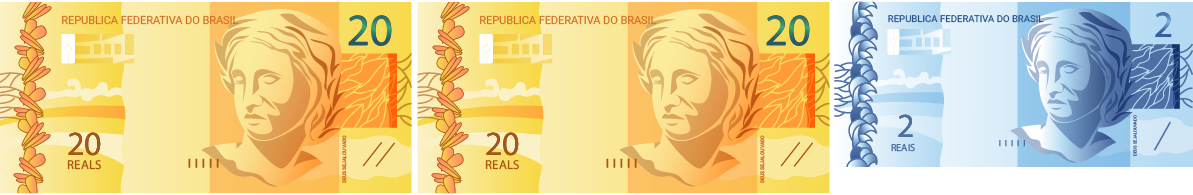
\includegraphics[width=\textwidth]{./media/SAEB_1ANO_MAT_FIGURA117b.png}
\end{figure}

QUE VALOR SOMAM AS CÉDULAS?

\begin{escolha}
\item R\$ 22,00.

\item R\$ 25,00.

\item R\$ 42,00.

\item R\$ 45,00.
\end{escolha}

\pagebreak
\num{10} ÉRICA COMPROU UM PACOTE DE BISCOITOS POR 10 REAIS. A MELHOR
FORMA DE PAGAR POR ESSE PRODUTO É COM DUAS CÉDULAS DE

\begin{escolha}
\item 5 REAIS.

\item 10 REAIS.

\item 20 REAIS.

\item 50 REAIS.
\end{escolha}

\vspace{1cm}

\num{11} QUAL DESTES EVENTOS É IMPOSSÍVEL DE ACONTECER?

\begin{escolha}
\item UMA FORMIGA TECER UMA TEIA.

\item UMA GAIVOTA VOAR SOBRE AS ÁGUAS DO MAR.

\item UM MACACO PULAR DE UM GALHO PARA OUTRO.

\item UM RINOCERONTE SER MUITO PESADO.
\end{escolha}

\vspace{1cm}

\num{12} INDIQUE QUAL DESTES ACONTECIMENTOS É CERTO DURANTE UM DIA.

\begin{escolha}
\item SENTIR ALEGRIA.

\item SENTIR FOME.

\item SENTIR DOR.

\item SENTIR TRISTEZA.
\end{escolha}

\pagebreak
\num{13} ANALISE O GRÁFICO.

\begin{figure}[H]
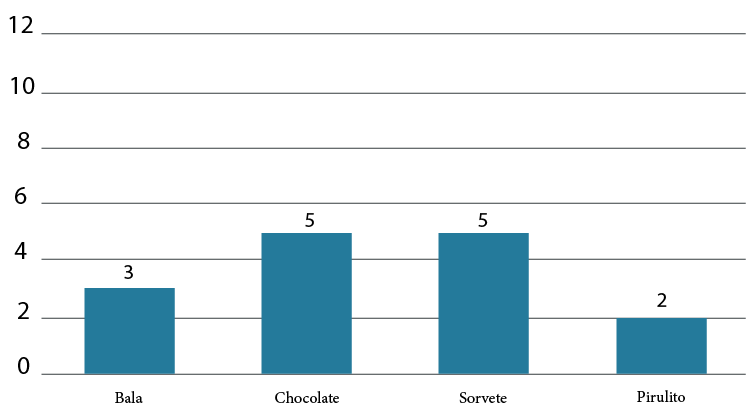
\includegraphics[width=\textwidth]{./media/SAEB_1ANO_MAT_FIGURA118.png}
\end{figure}

QUAIS SÃO OS DOIS DOCES PREFERIDOS DAS PESSOAS ENTREVISTADAS.

\begin{multicols}{2}
\begin{escolha}[itemsep=0pt]
\item BALA E CHOCOLATE.

\item CHOCOLATE E SORVETE.

\item PIRULITO E BALA.

\item SORVETE E PIRULITO.
\end{escolha}
\end{multicols}

\num{14} NA TABELA A SEGUIR, ESTÁ UMA LISTA DE COMPRAS COM OS PREÇOS PAGOS.

\begin{table}[!ht]
    \centering
    \begin{tabular}{|l|l|}
    \hline
        \textbf{ITEM} & \textbf{VALOR} \\ \hline
        DETERGENTE & 2 REAIS \\ \hline
        AMACIANTE DE ROUPA & 20 REAIS \\ \hline
        SABÃO EM PÓ & 15 REAIS \\ \hline
        DESINFETANTE & 18 REAIS \\ \hline
    \end{tabular}
\end{table}

% \begin{figure}[H]
% 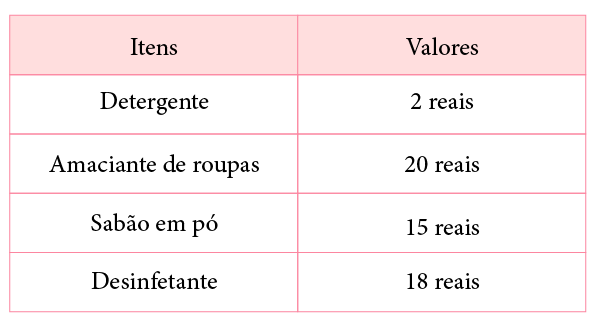
\includegraphics[width=\textwidth]{./media/SAEB_1ANO_MAT_FIGURA120.png}
% \end{figure}

O PRODUTO COM MENOR PREÇO É O

\begin{multicols}{2}
\begin{escolha}[itemsep=0pt]
\item AMACIANTE DE ROUPA.

\item DETERGENTE.

\item DESINFETANTE.

\item SABÃO EM PÓ.
\end{escolha}
\end{multicols}

\pagebreak
\num{15} A TABELA A SEGUIR MOSTRA AS TEMPERATURAS DE UM PERÍODO DE MUITO FRIO NO ESTADO DE SÃO
PAULO, EM 2017. OBSERVE.

%\textless{}inserir a tabela a seguir com referência: https://www.climatempo.com.br/noticia/2017/08/06/sao-paulo-esquenta-nesta-semana-7566. Colocar as letras em caixa alta e eliminar a segunda casa da vírgula, mantendo somente o número inteiro.\textgreater{}

\begin{figure}[H]
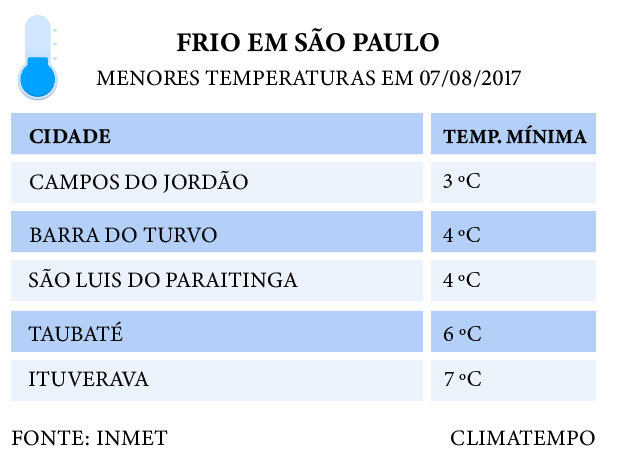
\includegraphics[width=\textwidth]{./media/SAEB_1ANO_MAT_FIGURA119.png}
\end{figure}

INDIQUE QUAL DESSAS CIDADES FICOU MAIS FRIA NESSE PERÍODO.

\begin{escolha}
\item BARRA DO TURVO.

\item CAMPOS DO JORDÃO.

\item ITUVERAVA.

\item TAUBATÉ.
\end{escolha}

\pagebreak


%\blankpage

%\vspace*{-3.4cm}
%\hspace*{-3.7cm}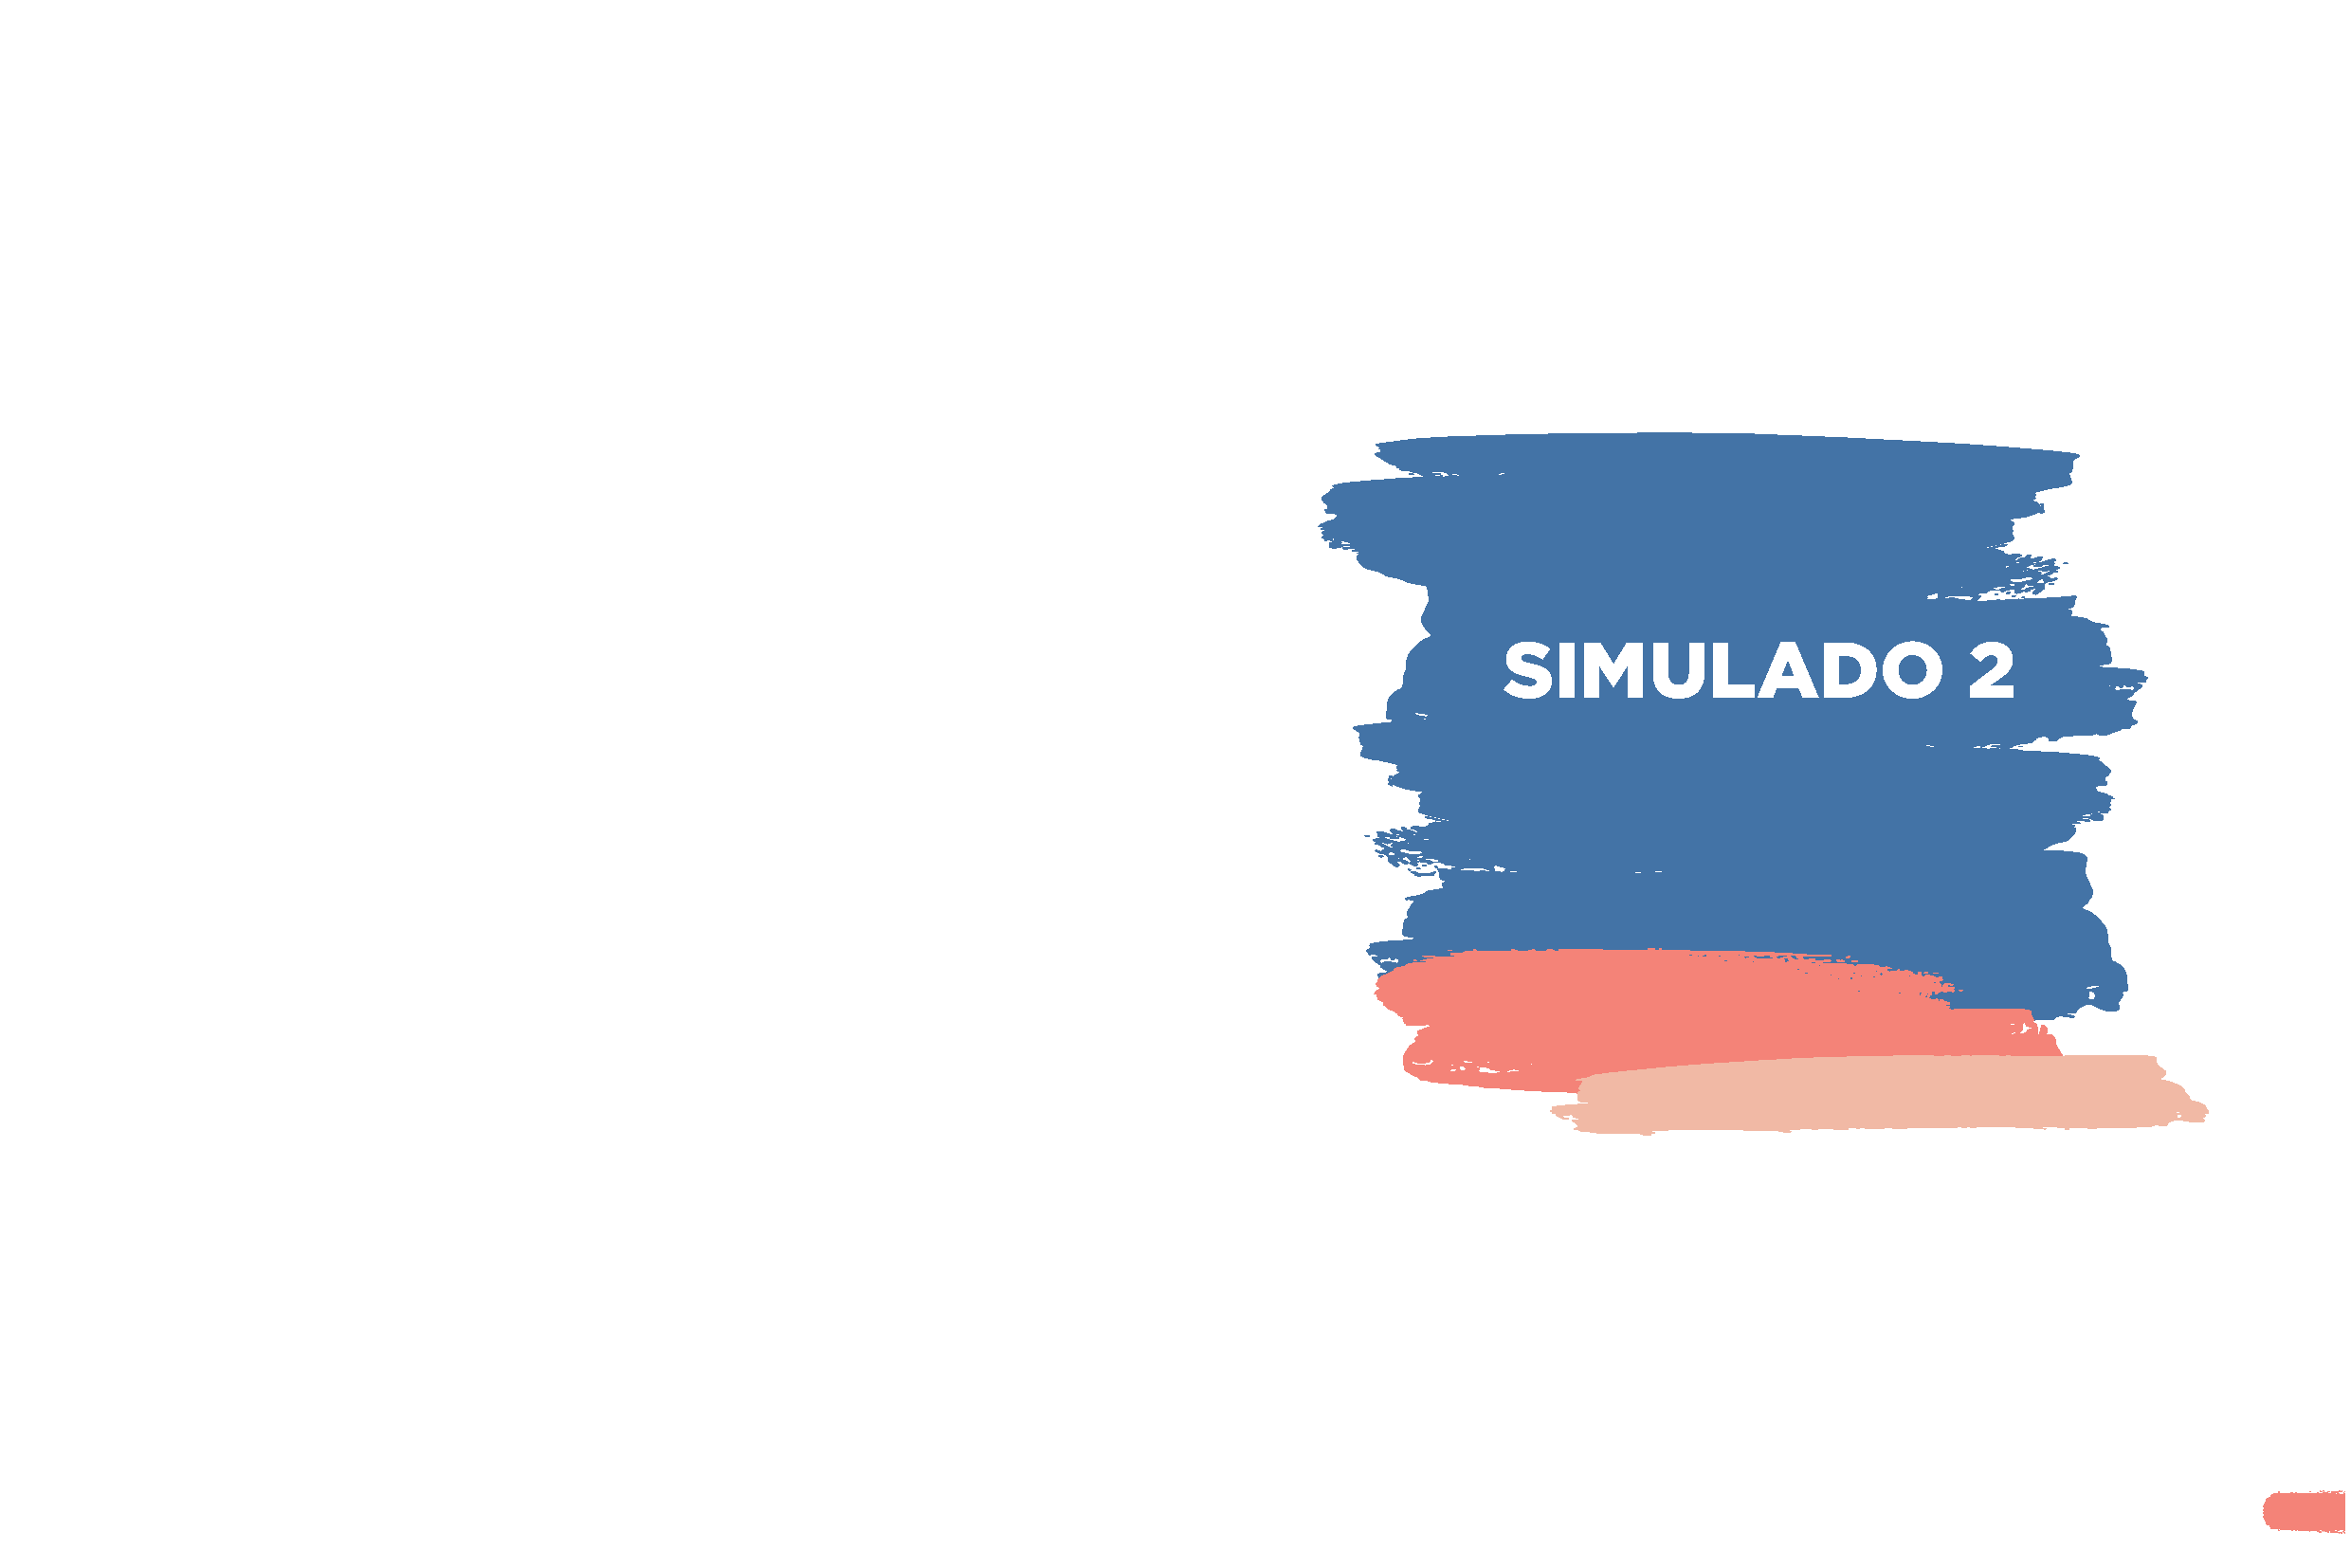
\includegraphics[scale=1]{../watermarks/2simulado5ano.pdf}

\addcontentsline{toc}{chapter}{SIMULADO 2}
\markboth{Simulado 2}{}

\num{1} LEIA O TEXTO.

\begin{myquote}
ACREDITA-SE QUE MAIS DE SETECENTOS E OITENTA E QUATRO ANIMAIS JÁ
DEIXARAM DE EXISTIR POR CAUSA DOS SERES HUMANOS.
\end{myquote}

ESCRITO EM ALGARISMOS, O NÚMERO QUE APARECE NESSE TEXTO É

\begin{escolha}
\item 478.

\item 487.

\item 784.

\item 874.
\end{escolha}

\num{2} OBSERVE ESTA LISTA DE NOMES COM AS IDADES DAS RESPECTIVAS PESSOAS.

\begin{myquote}
\begin{itemize}
  \item MARCOS -- 25 ANOS;
  \item CLÁUDIO -- 20 ANOS;
  \item HENRIQUE -- 18 ANOS;
  \item ANTÔNIO -- 45 ANOS.
\end{itemize}
\end{myquote}

QUAL DESSAS PESSOAS NASCEU PRIMEIRO?

\begin{escolha}
\item ANTÔNIO.

\item CLÁUDIO.

\item HENRIQUE.

\item MARCOS.
\end{escolha}

\pagebreak
\num{3} DOIS AMIGOS FAZEM COLEÇÃO DE MOEDAS. A COLEÇÃO DE JOSÉ ESTÁ REPRESENTADA NA IMAGEM DA
ESQUERDA. A COLEÇÃO DE JOÃO ESTÁ REPRESENTADA NA IMAGEM DA DIREITA.

%\textless{}https://br.freepik.com/vetores-gratis/moedas-de-ouro-com simbolos\_754238.htm\#query=moedas\%20cole\%C3\%A7\%C3\%A3o\&position=19\&from\_view=search\&track=ais;. https://br.freepik.com/vetores-gratis/simbolos-das-moedas-principais-representados-como-moedas-de-ouro\_1311029.htm\#query=moedas\%20cole\%C3\%A7\%C3\%A3o\&position=10\&from\_view=search\&track=ais.\textgreater{}

\begin{figure}[H]
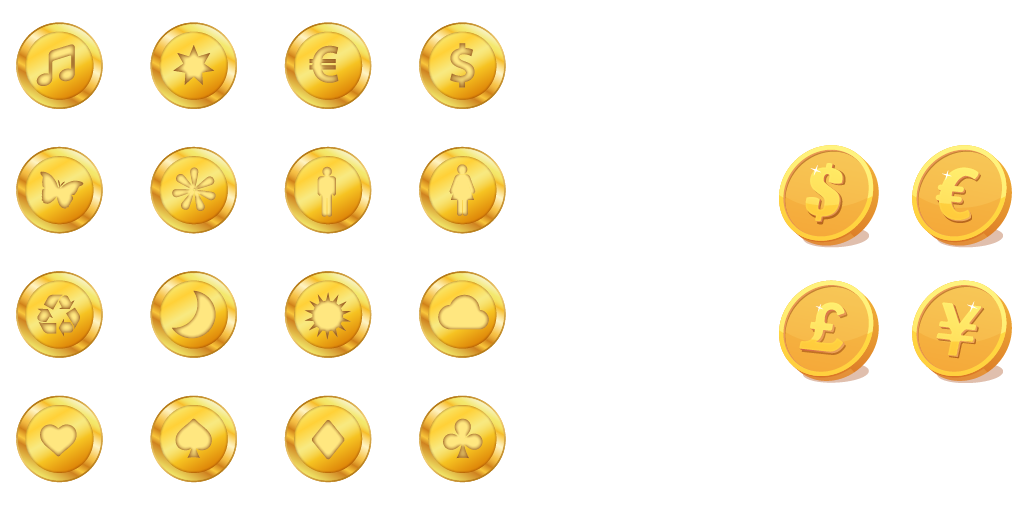
\includegraphics[width=\textwidth]{./media/SAEB_1ANO_MAT_FIGURA121.png}
\end{figure}

JOSÉ E JOÃO RESOLVERAM IGUALAR SUAS COLEÇÕES PARA QUE AMBOS FIQUEM COM O MESMO NÚMERO DE MOEDAS. QUANTAS MOEDAS JOSÉ DEVE DAR A JOÃO COM ESSE OBJETIVO?

\begin{escolha}[itemsep=0pt]
\item 6.

\item 10.

\item 12.

\item 20.
\end{escolha}

\num{4} ENTRE AS ADIÇÕES QUE APARECEM A SEGUIR, A ADIÇÃO QUE 
TEM COMO RESULTADO O NÚMERO \textbf{64} É

\begin{escolha}[itemsep=0pt]
\item 15 + 15 + 15 + 15.

\item 16 + 16 + 16 + 16.

\item 17 + 17 + 17 +17.

\item 18 + 18 + 18 + 18.
\end{escolha}

\pagebreak
\num{5} CADA MARCAÇÃO DO MEDIDOR REPRESENTADO A SEGUIR MEDE 1 LITRO DE CAPACIDADE. OBSERVE.

%\textless{}https://br.freepik.com/icones-gratis/copo-de-medicao\_14680733.htm?query=medir\%20massa\%20de\%20l\%C3\%ADquidos\#from\_view=detail\_alsolike\textgreater{}

\begin{figure}[H]
\centering

\includegraphics[width=.2\textwidth]{media/image113.png}
\end{figure}

QUANTOS LITROS DE LÍQUIDO FALTAM PARA ENCHER O MEDIDOR?

\begin{escolha}[itemsep=0pt]
\item 1.

\item 2.

\item 3.

\item 5.
\end{escolha}

\num{6} OBSERVE A IMAGEM.

%\textless{} https://br.freepik.com/vetores-premium/balancas-de-cozinha\_4667621.htm\#query=balan\%C3\%A7a\&position=14\&from\_view=search\&track=sph.\textgreater{}

\begin{figure}[H]
\centering

\includegraphics[width=.25\textwidth]{./media/SAEB_1ANO_MAT_FIGURA123.png}
\end{figure}

QUE UNIDADE DE MEDIDA É USADA PELO INSTRUMENTO REPRESENTADO NA IMAGEM?

\begin{escolha}[itemsep=0pt]
\item CENTÍMETRO.

\item LITRO.

\item METRO.

\item QUILOGRAMA.
\end{escolha}

\pagebreak
\num{7} JÉSSICA FOI AO DENTISTA NO DIA 2 DE MARÇO, E O DENTISTA MARCOU SEU
RETORNO PARA O DIA 30 DE ABRIL. MARÇO TEM 31 DIAS, E ABRIL TEM 30 DIAS. EM QUANTOS DIAS JÉSSICA VAI VOLTAR AO DENTISTA?

\begin{escolha}
\item 29.

\item 30.

\item 59.

\item 60.
\end{escolha}

\num{8} UM TREM DA FERROVIA TRANSNORDESTINA PARTE DA ESTAÇÃO DE SUAPE (PE) ÀS 10:30 
HORAS DE UM DIA E, GERALMENTE, CHEGA À PRÓXIMA ESTAÇÃO, EM CACHOEIRINHA (PE), ÀS 
18:00 HORAS DO MESMO DIA. QUAL É A DURAÇÃO DA VIAGEM NESSE TRECHO?

\begin{escolha}
\item 6 HORAS.

\item 7 HORAS E 30 MINUTOS.

\item 8 HORAS.

\item 8 HORAS E 30 MINUTOS.
\end{escolha}

\num{9} OBSERVE A IMAGEM.

%\textless{}https://br.freepik.com/fotos-gratis/dinheiro-moedas-brasileiras-1-real\_22809605.htm\#query=moeda\%20de\%201\%20real\%20dineiro\%20barssileiro\&position=1\&from\_view=search\&track=ais\textgreater{}

\begin{figure}[H]
\centering
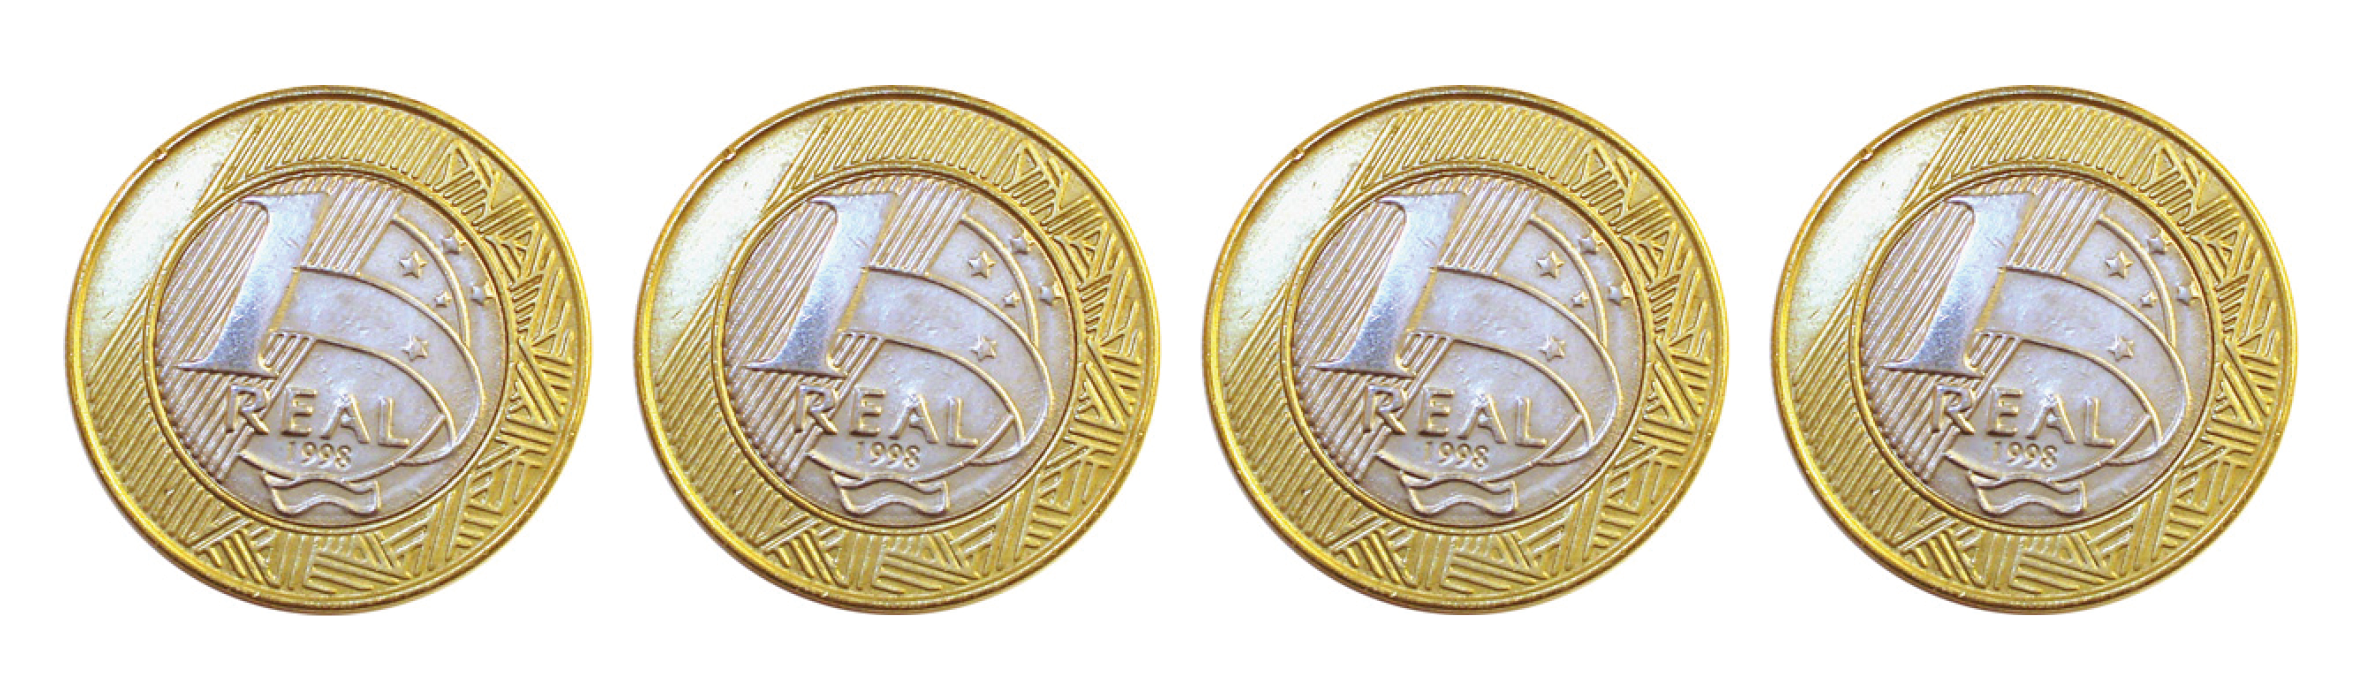
\includegraphics[width=.6\textwidth]{./media/SAEB_1ANO_MAT_FIGURA124.png}
\end{figure}

QUE VALOR ESTÁ REPRESENTADO NA IMAGEM?

\begin{multicols}{2}
\begin{escolha}
\item R\$ 1,00.

\item R\$ 2,00.

\item R\$ 3,00.

\item R\$ 4,00.
\end{escolha}
\end{multicols}

\num{10} JUCA TEM CINCO CÉDULAS DE R\$ 10,00. COM ESSE VALOR, ELE CONSEGUE COMPRAR

\begin{multicols}{2}
\begin{escolha}[itemsep=0pt]
\item UMA BOLA DE R\$ 65,00.

\item UM CARRINHO DE R\$ 35,00.

\item UMA BONECA DE R\$ 52,00.

\item UM JOGO DE R\$ 85,00.
\end{escolha}
\end{multicols}

\num{11} QUAL DESTES ACONTECIMENTOS É POUCO PROVÁVEL?

\begin{escolha}[itemsep=0pt]
\item A LUA APARECER NO CÉU À NOITE.

\item O SOL NASCER NO CÉU DE MANHÃ.

\item UM CARRO PASSAR POR UMA RUA DE UMA CIDADE.

\item UMA LAGARTIXA SUBIR PELAS COSTAS DE ALGUÉM.
\end{escolha}

\num{12} O GRÁFICO MOSTRA A COLEÇÃO DE BRINQUEDOS DE JOÃO. CADA FIGURA DE UM
BRINQUEDO REPRESENTA UMA UNIDADE. OBSERVE.

\begin{figure}[H]
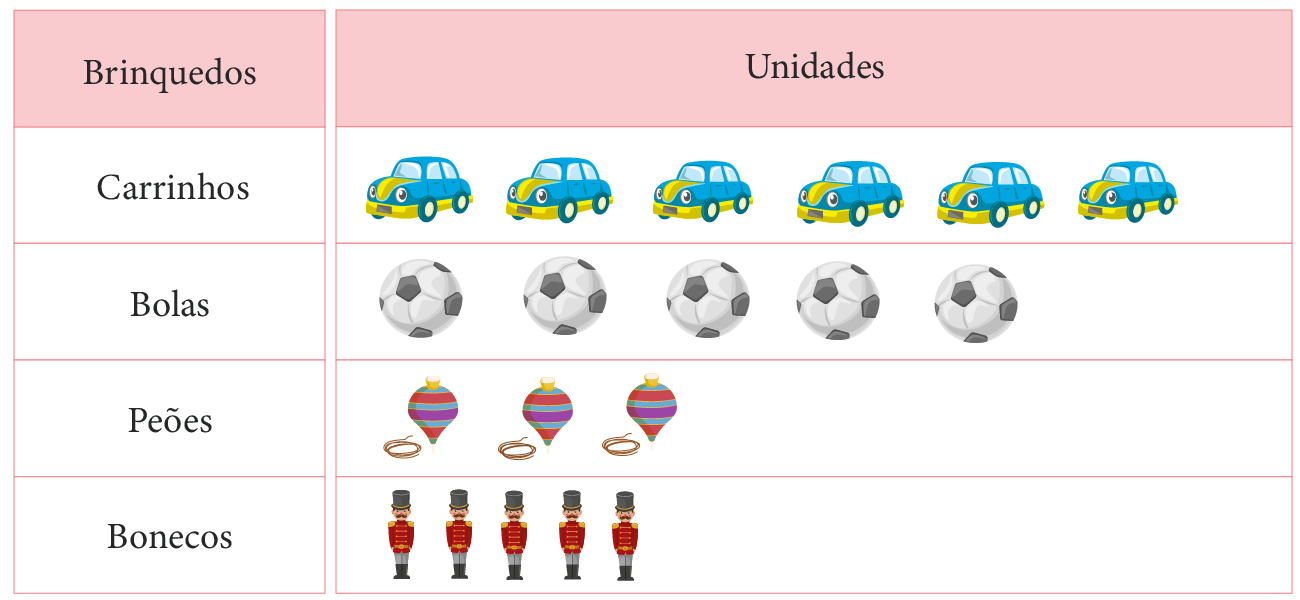
\includegraphics[width=\textwidth]{./media/SAEB_1ANO_MAT_FIGURA126.png}
\end{figure}

ELE TEM NA MESMA QUANTIDADE

\begin{multicols}{2}
\begin{escolha}[itemsep=0pt]
\item BOLAS E BONECOS.

\item BOLAS E CARRINHOS.

\item CARRINHOS E PEÕES.

\item PEÕES E BONECOS.
\end{escolha}
\end{multicols}

\pagebreak

\num{13} INDIQUE QUAL DAS IMAGENS REPRESENTA UMA CENA POSSÍVEL.

%\textless{}As referências são: https://br.freepik.com/vetores-gratis/tiranossauro-rex-dinossauro-dancando-bale-no-estilo-cartoon\_26348697.htm\#query=jacar\%C3\%A9\%20vestido\&position=2\&from\_view=search\&track=ais; https://br.freepik.com/vetores-premium/leao-dos-desenhos-animados-pulando-atraves-do-anel\_3245417.htm\#query=le\%C3\%A3o\%20malabarista\&position=6\&from\_view=search\&track=ais; https://br.freepik.com/vetores-gratis/tubarao-bebendo-vinho-na-ilha\_32541982.htm\#query=passarinho\%20surfando\&position=1\&from\_view=search\&track=ais;

\begin{multicols}{2}
\begin{escolha}
\item 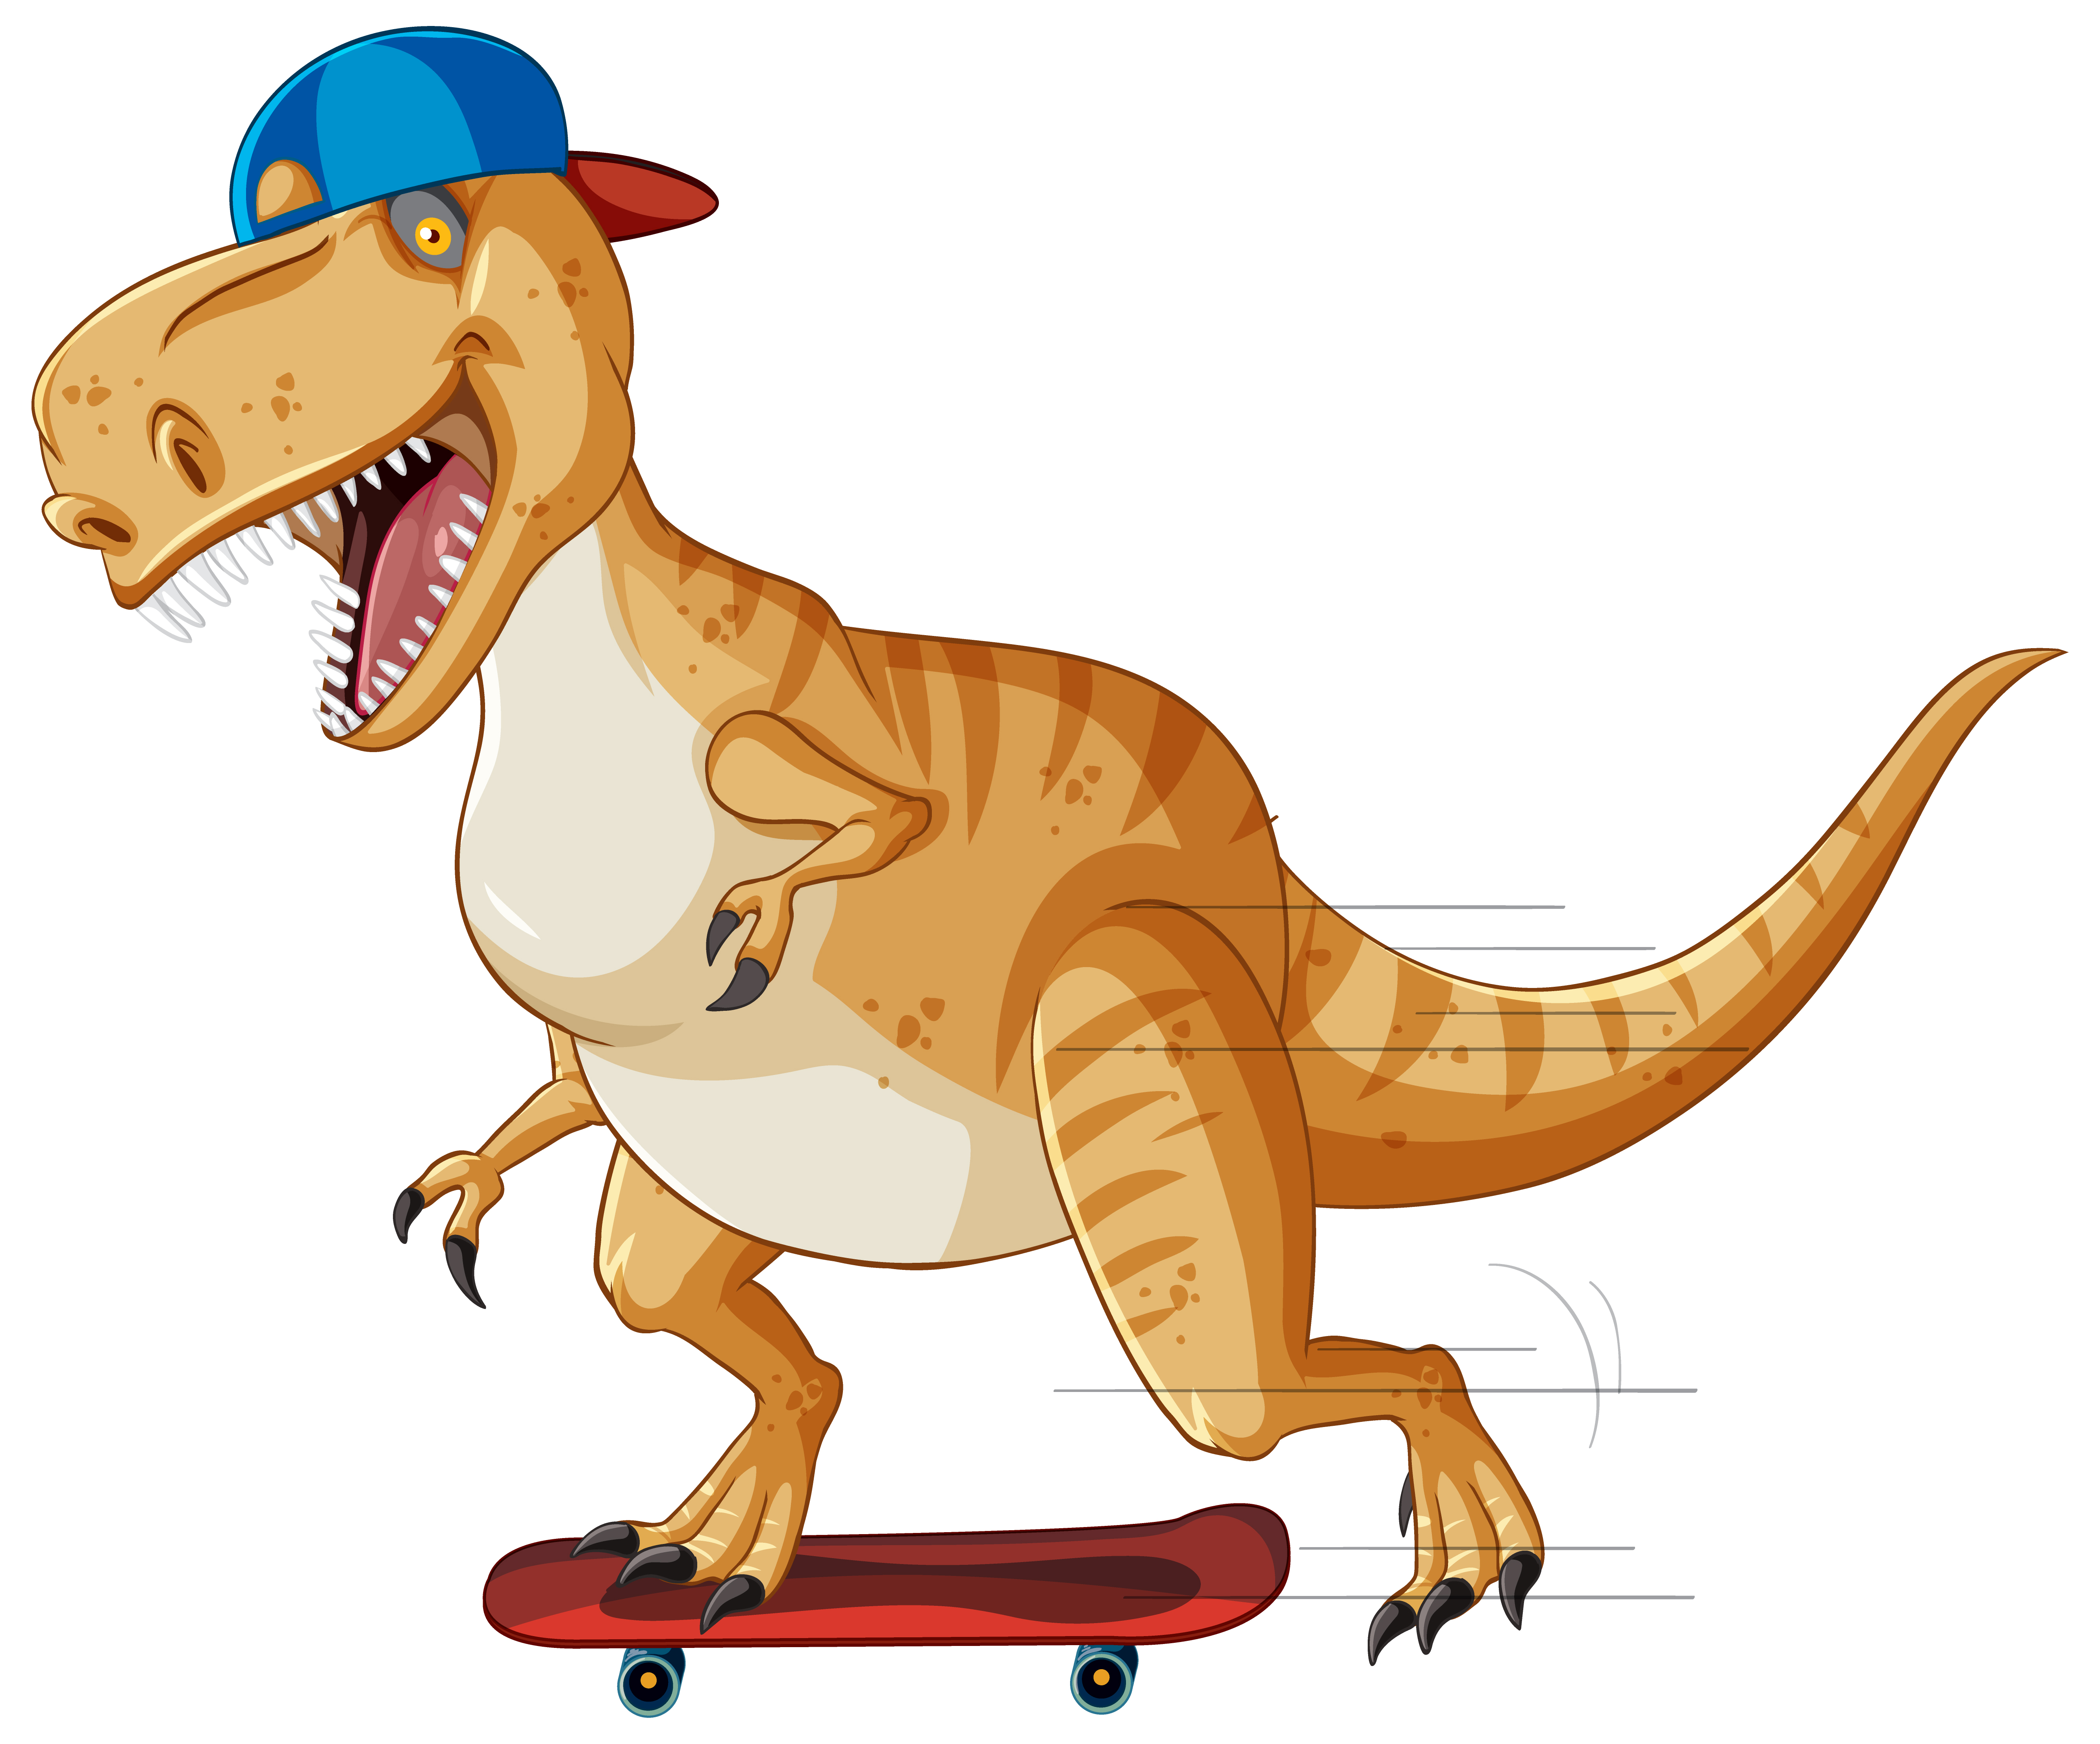
\includegraphics[width=.3\textwidth]{./media/SAEB_1ANO_MAT_FIGURA125a.jpg}
\item 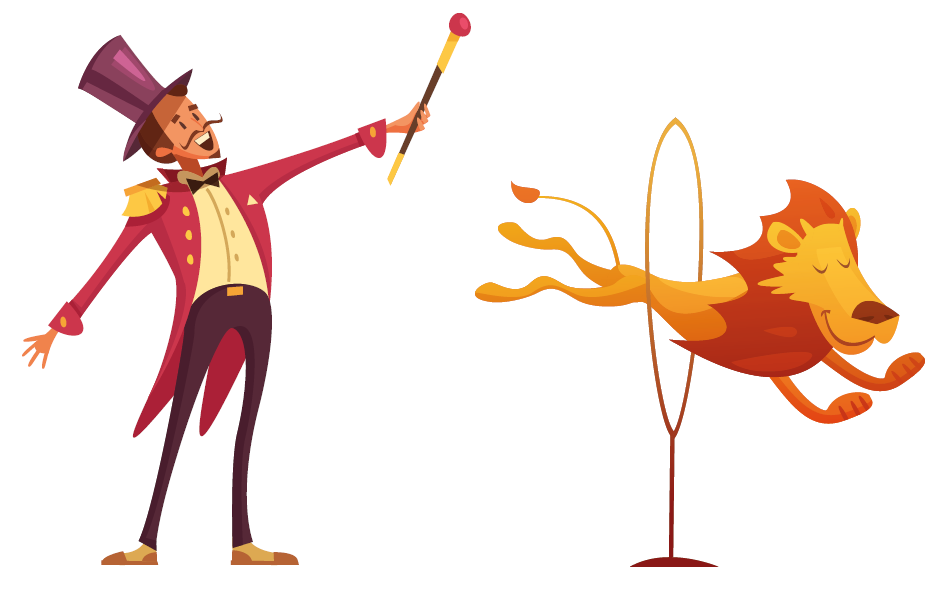
\includegraphics[width=.3\textwidth]{./media/SAEB_1ANO_MAT_FIGURA125b.png}

\columnbreak

\item 
\includegraphics[width=.3\textwidth]{./media/SAEB_1ANO_MAT_FIGURA125c.png}
\item 
\includegraphics[width=.3\textwidth]{./media/SAEB_1ANO_MAT_FIGURA125d.png}
\end{escolha}
\end{multicols}


\num{14} ANALISE O GRÁFICO E ASSINALE QUANDO VAI CHOVER.

%\textless{}INSERIR TABELA COM OS ÍCONES DA REFERÊNCIA: https://br.freepik.com/vetores-gratis/icones-da-linha-do-tempo\_946338.htm\#query=\%C3\%ADcones\%20do\%20clima\&position=34\&from\_view=search\&track=ais, conforme o modelo a seguir.\textgreater{}

\begin{figure}[H]
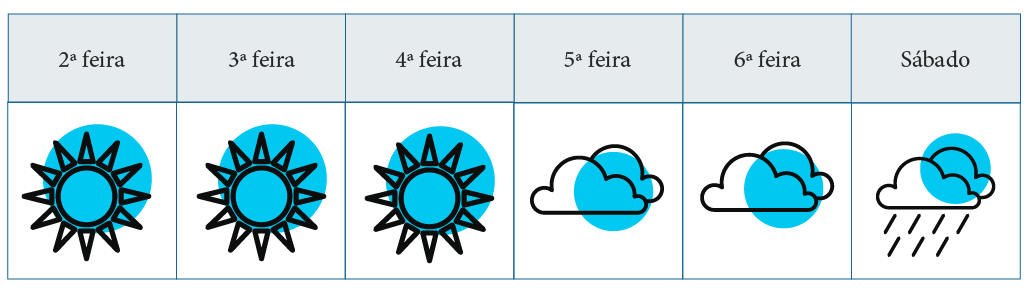
\includegraphics[width=\textwidth]{./media/SAEB_1ANO_MAT_FIGURA127.png}
\end{figure}

\begin{escolha}[itemsep=0pt]
\item SEGUNDA-FEIRA.

\item TERÇA-FEIRA.

\item QUARTA-FEIRA.

\item QUINTA-FEIRA.
\end{escolha}

\num{15} A TABELA MOSTRA COMO ESTÃO QUATRO AMIGOS. OBSERVE.

%\textless{}inserir as figuras da referência: https://br.freepik.com/vetores-gratis/whatsapp-emoji\_904078.htm\#query=emojis\&position=3\&from\_view=search\&track=sph, na tabela, conforme o modelo a seguir.\textgreater{}

\begin{figure}[H]
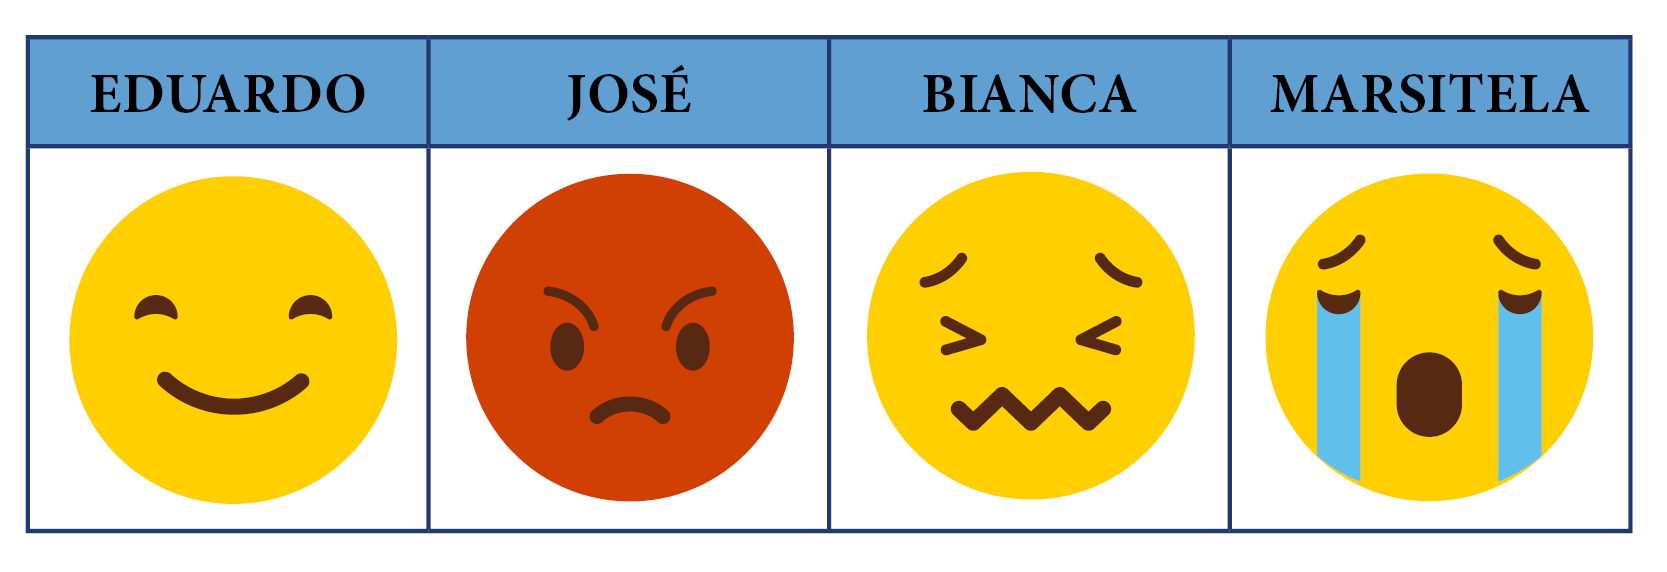
\includegraphics[width=\textwidth]{./media/SAEB_1ANO_MAT_FIGURA128.png}
\end{figure}

QUAL DELES ESTÁ FELIZ?

\begin{escolha}[itemsep=0pt]
\item BIANCA.

\item EDUARDO.

\item JOSÉ.

\item MARISTELA.
\end{escolha}

\pagebreak

%\blankpage

%\vspace*{-3.4cm}
%\hspace*{-3.7cm}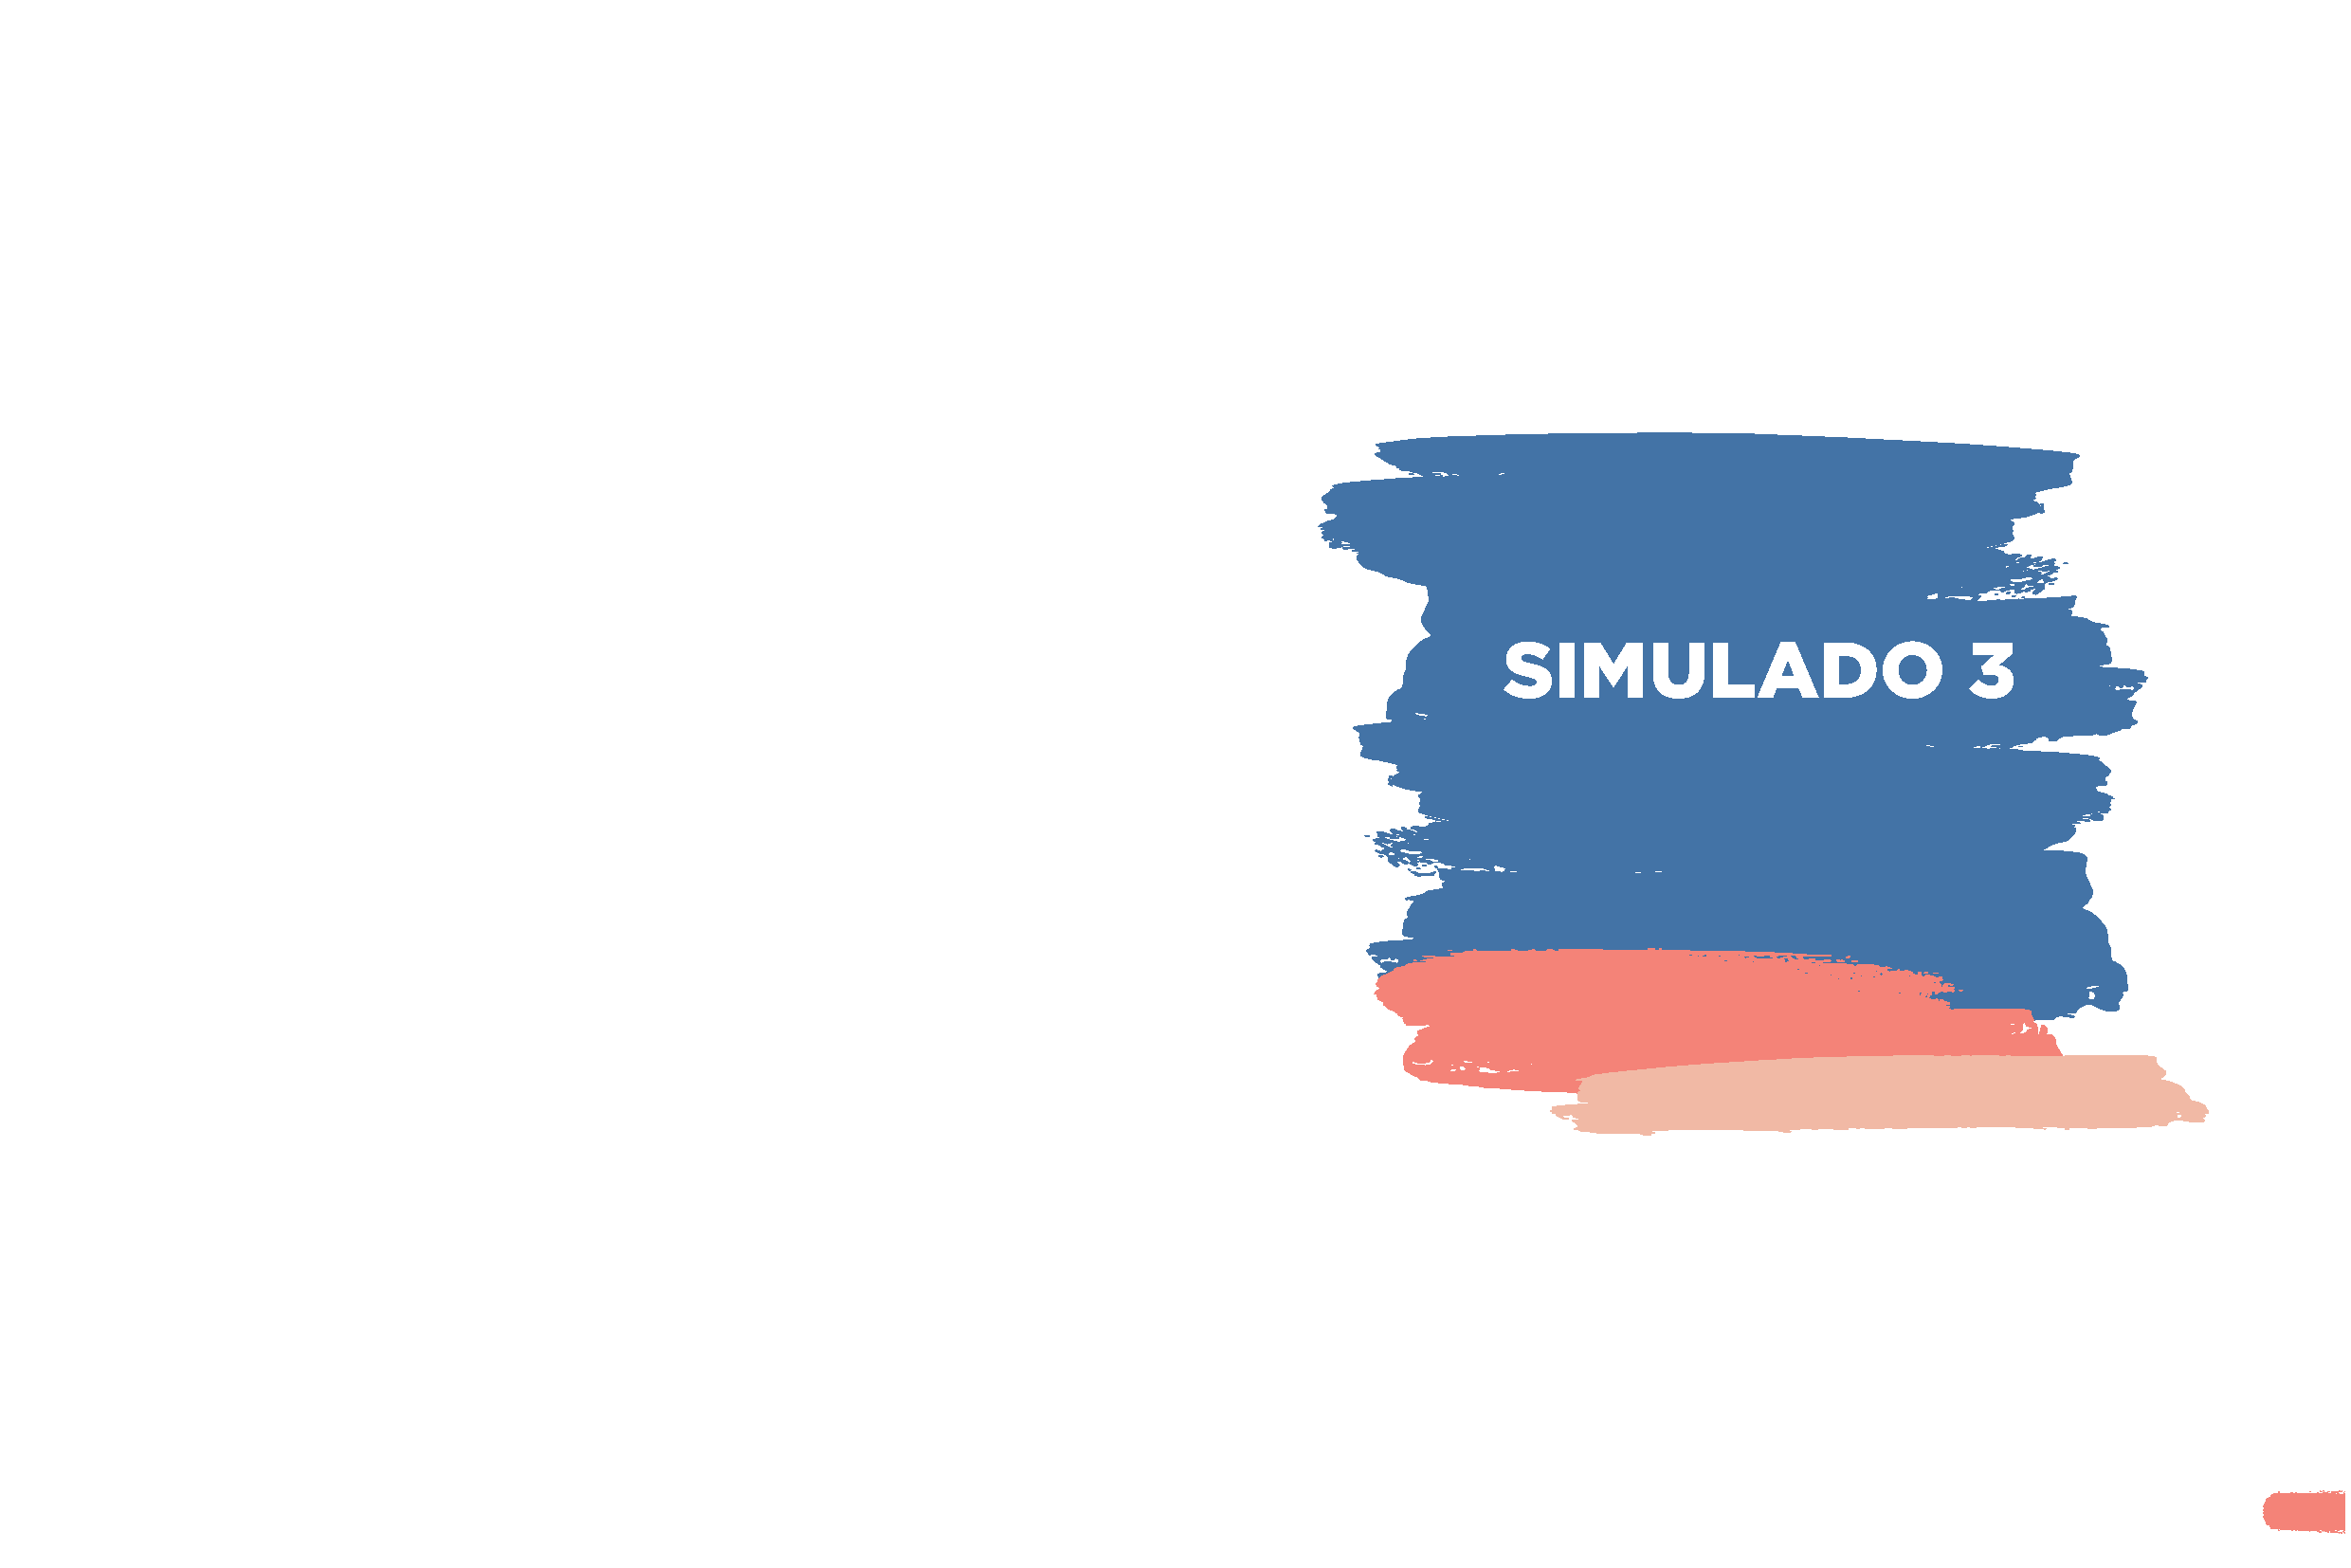
\includegraphics[scale=1]{../watermarks/3simulado5ano.pdf}

\addcontentsline{toc}{chapter}{SIMULADO 3}
\markboth{Simulado 3}{}

\num{1} OBSERVE ESTA LISTA DE ESTADOS BRASILEIROS COM OS RESPECTIVOS NÚMEROS DE MUNICÍPIOS.

\begin{itemize}
  \item \textbf{BAHIA}: 417 MUNICÍPIOS;
  \item \textbf{AMAZONAS}: 62 MUNICÍPIOS;
  \item \textbf{CEARÁ}: 184 MUNICÍPIOS;
  \item \textbf{MINAS GERAIS}: 853 MUNICÍPIOS.
\end{itemize}

SE ESSA LISTA FOR ORGANIZADA EM ORDEM CRESCENTE, O PRIMEIRO ESTADO DA LISTA SERÁ

\begin{escolha}[itemsep=0pt]
\item A BAHIA.

\item O AMAZONAS.

\item O CEARÁ.

\item MINAS GERAIS.
\end{escolha}

\num{2} QUANTAS CENTENAS TEM O NÚMERO 999?

\begin{escolha}[itemsep=0pt]
\item 0.

\item 9.

\item 90.

\item 900.
\end{escolha}

\num{3} DOIS TIMES DISPUTARAM UMA PARTIDA DE FUTEBOL. FORAM FEITOS 15 GOLS NESSA
PARTIDA. O TIME B VENCEU O TIME A. INDIQUE QUAL DOS RESULTADOS ABAIXO É
POSSÍVEL?

\begin{escolha}[itemsep=0pt]
\item TIME A 8 X 7 TIME B.

\item TIME A 6 X 9 TIME B.

\item TIME A 11 X 5 TIME B.

\item TIME A 0 X 14 TIME B.
\end{escolha}

\pagebreak
\num{4} COMBINE AS CÉDULAS DE FORMA A INTEIRAR R\$ 35,00. ESCOLHA A OPÇÃO CORRETA.

\begin{escolha}
\item 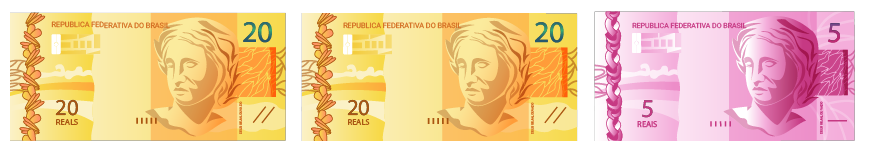
\includegraphics[width=\textwidth]{./media/SAEB_1ANO_MAT_FIGURA129a.png}
\item 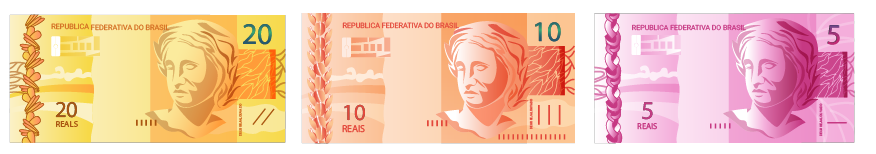
\includegraphics[width=\textwidth]{./media/SAEB_1ANO_MAT_FIGURA129b.png}
\item 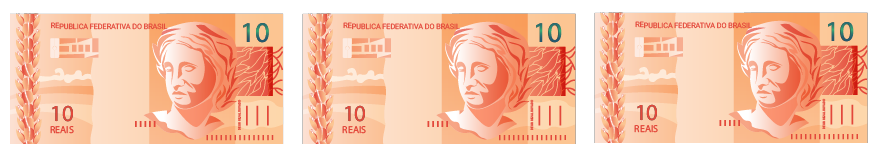
\includegraphics[width=\textwidth]{./media/SAEB_1ANO_MAT_FIGURA129c.png}
\item 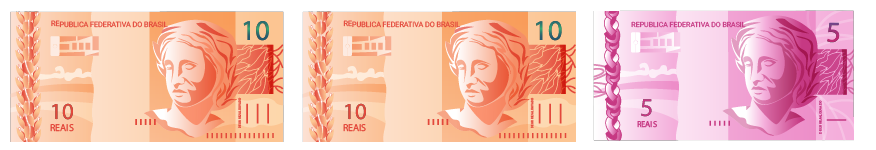
\includegraphics[width=\textwidth]{./media/SAEB_1ANO_MAT_FIGURA129d.png}
\end{escolha}

\num{5} ANALISE A IMAGEM COM VÁRIAS VISTAS DO MESMO CARRO.

%\textless{} https://br.freepik.com/vetores-gratis/carro-moderno-em-diferentes-vistas\_1358025.htm\#query=carros\%20de\%20tamanhos\%20diferentes\&position=13\&from\_view=search\&track=ais. Retire o texto em inglês.\textgreater{}


\begin{figure}[H]
\centering
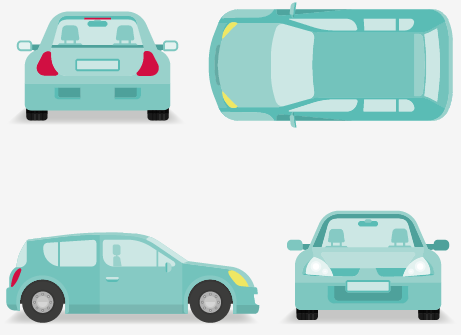
\includegraphics[width=.6\textwidth]{./media/SAEB_1ANO_MAT_FIGURA130.png}
\end{figure}

É CORRETO AFIRMAR QUE O CARRO PARECE MAIOR QUANDO VISTO DE

\begin{multicols}{2}
\begin{escolha}
\item CIMA.

\item FRENTE.

\item QUALQUER LADO.

\item TRÁS.
\end{escolha}
\end{multicols}


\num{6} OBSERVE A REPRESENTAÇÃO DE ALGUNS BICHOS.
QUAL DESTES ANIMAIS DEVE TER A MENOR MASSA?

%\textless{}Referências: https://br.freepik.com/vetores-gratis/elefante-adulto-sem-marfim-em-estilo-cartoon-sobre-fundo-branco\_12321510.htm\#query=elefante\&position=6\&from\_view=search\&track=sph; https://br.freepik.com/vetores-gratis/projeto-do-tigre-colorido\_956292.htm\#page=2\&query=tigre\&position=6\&from\_view=search\&track=sph; https://br.freepik.com/vetores-premium/mascote-crocodilo-em-corpo-inteiro\_19627455.htm\#page=2\&query=jacar\%C3\%A9\&position=13\&from\_view=search\&track=sph; https://br.freepik.com/vetores-premium/armadillo-no-fundo-branco\_1426695.htm?query=gamb\%C3\%A1\#from\_view=detail\_alsolike

\begin{multicols}{2}
\begin{escolha}
\item 
\includegraphics[width=.3\textwidth]{./media/SAEB_1ANO_MAT_FIGURA131a.png}
\item 
\includegraphics[width=.3\textwidth]{./media/SAEB_1ANO_MAT_FIGURA131b.png}

\columnbreak

\item 
\includegraphics[width=.3\textwidth]{./media/SAEB_1ANO_MAT_FIGURA131c.png}
\item 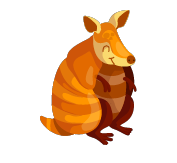
\includegraphics[width=.3\textwidth]{./media/SAEB_1ANO_MAT_FIGURA131d.png}
\end{escolha}
\end{multicols}

\num{7} JAQUELINE ENVIOU UMA ENCOMENDA PARA SUA AMIGA NA SEGUNDA-FEIRA. A ENCOMENDO CHEGOU 10 DIAS DEPOIS. EM QUE DIA
DA SEMANA A ENCOMENDA CHEGOU?

\begin{multicols}{2}
\begin{escolha}[itemsep=0pt]
\item SEGUNDA-FEIRA.

\item TERÇA-FEIRA.

\item QUARTA-FEIRA.

\item QUINTA-FEIRA.
\end{escolha}
\end{multicols}

\num{8} TRÊS DIAS DEPOIS DE UM SÁBADO É

\begin{escolha}[itemsep=0pt]
\item UM DOMINGO.

\item UMA SEGUNDA-FEIRA.

\item UMA TERÇA-FEIRA.

\item UMA QUARTA-FEIRA.
\end{escolha}

\num{9} OBSERVE A MOEDA REPRESENTADA A SEGUIR.

\begin{figure}[H]
\centering
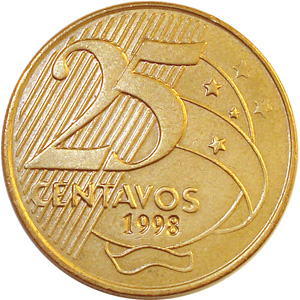
\includegraphics[width=.2\textwidth]{./media/SAEB_1ANO_MAT_FIGURA132.png}
\end{figure}

QUAL É O VALOR DESSA MOEDA?

\begin{multicols}{2}
\begin{escolha}[itemsep=0pt]
\item 10 CENTAVOS.

\item 25 CENTAVOS.

\item 50 CENTAVOS.

\item 1 REAL.
\end{escolha}
\end{multicols}



\num{10} BETO TEM EM DINHEIRO O VALOR REPRESENTADO A SEGUIR.

\begin{figure}[H]
\centering
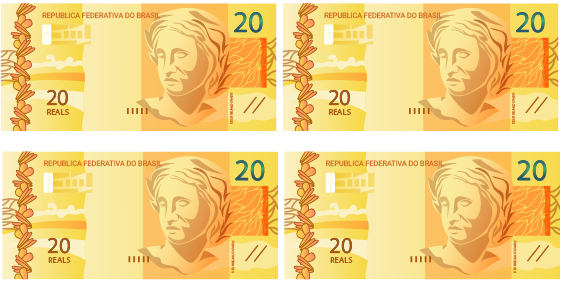
\includegraphics[width=\textwidth]{./media/SAEB_1ANO_MAT_FIGURA133b.png}
\end{figure}

A ÚNICA DESTAS PEÇAS DE ROUPA QUE ELE PODE COMPRAR COM ESSA QUANTIA É UMA

\begin{escolha}
\item CAMISA DE R\$ 110,00.

\item CALÇA DE R\$ 100,00.

\item CALÇA DE R\$ 90,00.

\item BERMUDA DE R\$ 60,00.
\end{escolha}

\num{11} QUAL DESTES SUPER-HERÓIS TEM HABILIDADES POSSÍVEIS PARA QUALQUER SER HUMANO?

\begin{multicols}{2}
\begin{escolha}
\item BATMAN.

\item HOMEM-ARANHA.

\item HOMEM-FORMIGA.

\item SUPER-HOMEM.
\end{escolha}
\end{multicols}


\num{12} ENTRE OS ACONTECIMENTOS A SEGUIR, QUAL NÃO É CERTEZA QUE VAI
ACONTECER?

\begin{escolha}[itemsep=-5pt]
\item CABELO CRESCER DEPOIS DE CORTAR.

\item MACHUCAR-SE DEPOIS DE CAIR.

\item SUAR DEPOIS DE CORRER MUITO.

\item UNHA CRESCER DEPOIS DE CORTAR.
\end{escolha}

\num{13} QUANDO ANOITECE, QUAL EVENTO A SEGUIR É CERTO?

\begin{escolha}[itemsep=-5pt]
\item A LUA PODERÁ SER VISTA.

\item AS ESTRELAS PODERÃO SER VISTAS.

\item O SOL NÃO PODERÁ SER VISTO.

\item CHUVA CAIRÁ DO CÉU.
\end{escolha}

\num{14} O GRÁFICO MOSTRA AS BRINCADEIRAS PREFERIDAS DAS CRIANÇAS DE UMA TURMA.

\begin{figure}[H]
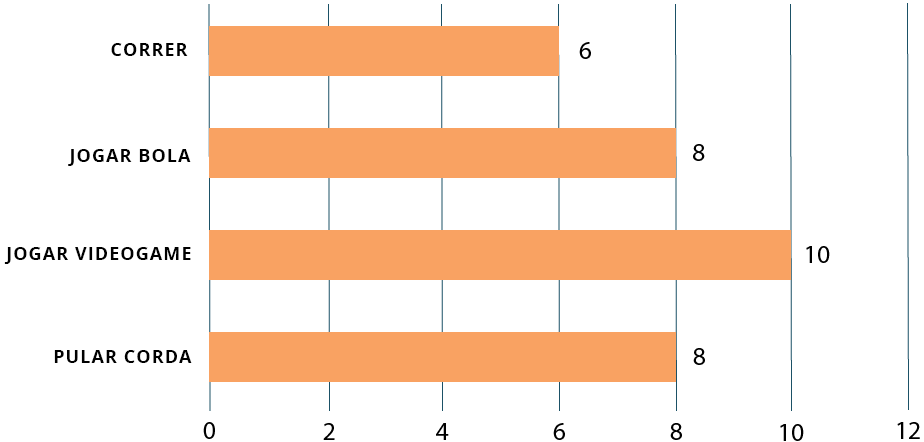
\includegraphics[width=\textwidth]{./media/SAEB_1ANO_MAT_FIGURA134.png}
\end{figure}

\pagebreak
QUAL É A BRINCADEIRA MENOS PRATICADA?

\begin{escolha}
\item CORRER.

\item JOGAR BOLA.

\item JOGAR \textit{VIDEOGAME}.

\item PULAR CORDA.
\end{escolha}

\num{15} A TABELA DESCREVE A COLEÇÃO DE LIVROS DE NÍCOLAS.

% \begin{figure}[htpb!]
% 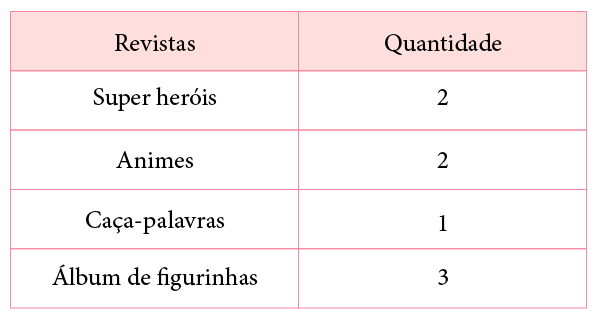
\includegraphics[width=\textwidth]{./media/SAEB_1ANO_MAT_FIGURA135.png}
% \end{figure}

\begin{table}[!ht]
    \centering
    \begin{tabular}{|l|l|}
    \hline
        \textbf{TIPO} & \textbf{QUANTIDADE} \\ \hline
        SUPER-HERÓI & 2 \\ \hline
        ANIME & 2 \\ \hline
        CAÇA-PALAVRA & 1 \\ \hline
        ÁLBUM DE FIGURINHA & 3 \\ \hline
    \end{tabular}
\end{table}

NO TOTAL, QUANTOS ITENS HÁ NA COLEÇÃO DE NÍCOLAS?

\begin{escolha}
\item 3.

\item 4.

\item 7.

\item 8.
\end{escolha}

%\vspace*{-3.4cm}
%\hspace*{-3.7cm}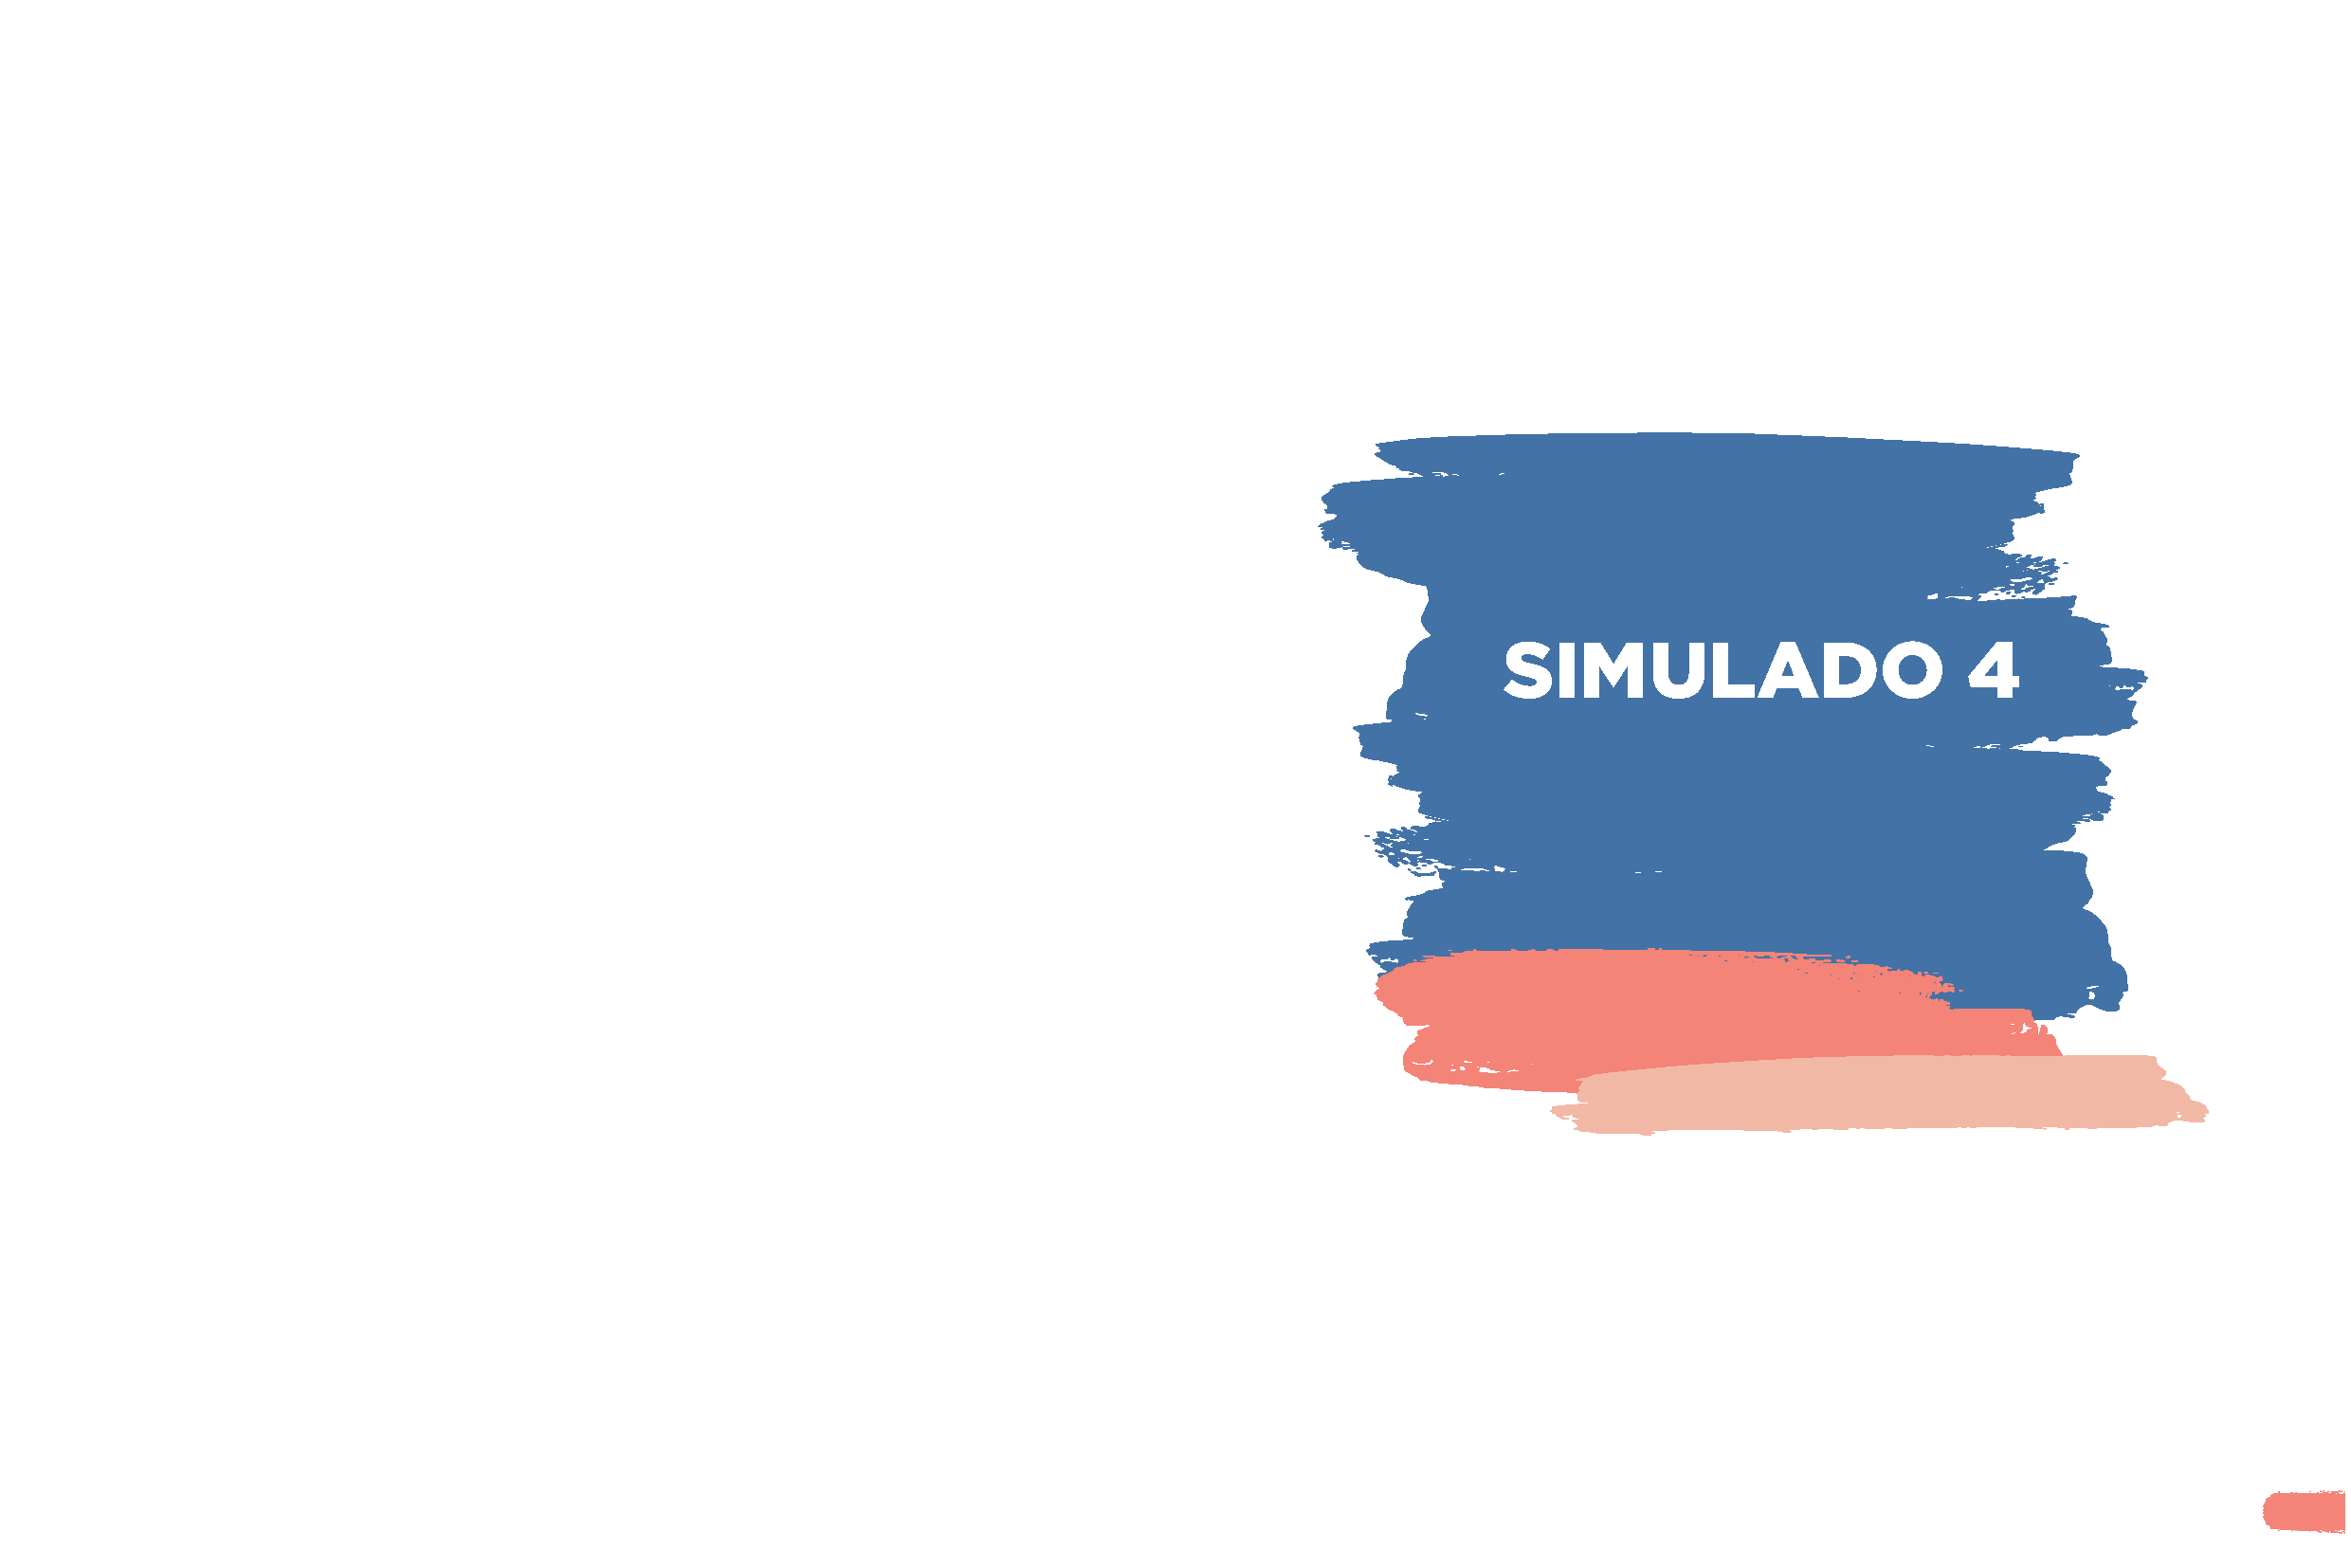
\includegraphics[scale=1]{../watermarks/4simulado5ano.pdf}

\pagebreak

\addcontentsline{toc}{chapter}{SIMULADO 4}
\markboth{Simulado 4}{}

\num{1} BIA COMPROU AS COMIDAS REPRESENTADAS
NA IMAGEM.

\begin{figure}[H]
\centering
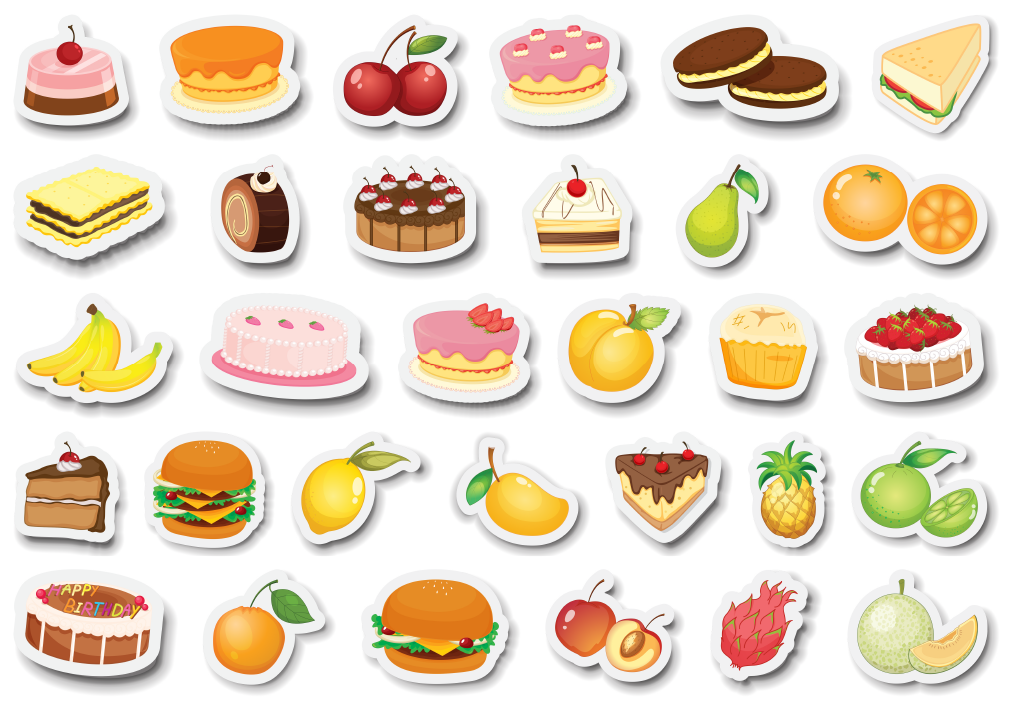
\includegraphics[width=\textwidth]{./media/SAEB_1ANO_MAT_FIGURA136.png}
\end{figure}

QUANTOS ITENS DE COMIDA SALGADA ELA COMPROU?

\begin{multicols}{4}
\begin{escolha}[itemsep=0pt]
\item 2.

\item 3.

\item 4.

\item 5.
\end{escolha}
\end{multicols}

\num{2} TRÊS AMIGOS ESTAVAM DISPUTANDO UMA CORRIDA. JONAS TERMINOU A CORRIDA EM 30
MINUTOS. MAURÍCIO TERMINOU A CORRIDA EM 25 MINUTOS. EVANDRO TERMINOU A
CORRIDA EM 45 MINUTOS. GANHOU A CORRIDA QUEM CHEGOU MAIS RÁPIDO AO FINAL. INDIQUE A
ORDEM CORRETA DO VENCEDOR ATÉ O ÚLTIMO LUGAR.

\begin{escolha}[itemsep=0pt]
\item EVANDRO --- JONAS --- MAURÍCIO.

\item EVANDRO --- MAURÍCIO --- JONAS.

\item JONAS --- MAURÍCIO --- EVANDRO

\item MAURÍCIO --- JONAS --- EVANDRO.
\end{escolha}

\pagebreak
\num{3} OBSERVE AS IMAGENS, QUE REPRESENTAM CAIXAS DE FRUTAS.

\begin{figure}[htpb!]
\centering
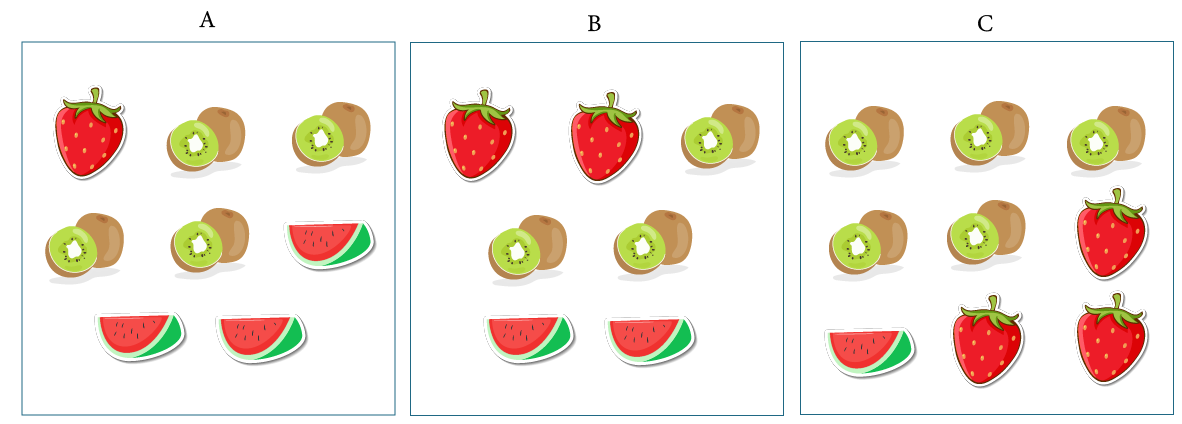
\includegraphics[width=\textwidth]{./media/SAEB_1ANO_MAT_FIGURA137.png}
\end{figure}

PARA QUE HAJA AS MESMAS QUANTIDADES DE FRUTAS NAS TRÊS CAIXAS, ALGO
A SE FAZER É TIRAR

\begin{escolha}[itemsep=0pt]
\item UM KIWI DA CAIXA \textbf{A} E PASSÁ-LA PARA A CAIXA \textbf{B}.

\item UMA MELANCIA DA CAIXA \textbf{C} E PASSÁ-LA PARA A CAIXA \textbf{B}.

\item UM MORANGO DA CAIXA \textbf{C} E PASSÁ-LA PARA A CAIXA \textbf{A}.

\item UMA MELANCIA DA CAIXA \textbf{A} E PASSÁ-LA PARA A CAIXA \textbf{B}.
\end{escolha}

\num{4} OBSERVE PARTE DE UMA LISTA DE MATERIAIS ESCOLARES COM OS PREÇOS.

\begin{myquote}
\begin{itemize}
  \item 300 FOLHAS DE PAPEL SULFITE: R\$ 23,00;
  \item 4 LÁPIS GRAFITE HB: R\$ 19,00;
  \item 2 BORRACHAS PEQUENAS: R\$ 8,00;
  \item CAIXA DE LÁPIS DE COR COM 24 LÁPIS: R\$ 43,00.
\end{itemize}
\end{myquote}


COM ESSA PARTE DA LISTA DE COMPRAS DE MATERIAL ESCOLAR, SERÃO GASTOS

\begin{multicols}{2}
\begin{escolha}[itemsep=0pt]
\item R\$ 42,00.

\item R\$ 50,00.

\item R\$ 51,00.

\item R\$ 93,00.
\end{escolha}
\end{multicols}

\num{5} QUAL DESTES INSTRUMENTOS É O MAIS ADEQUADO PARA MEDIR A QUANTIDADE DE SUCO EXTRAÍDO DE UMA DÚZIA DE LARANJAS?

\begin{multicols}{2}
\begin{escolha}[itemsep=0pt]
\item BALANÇA.

\item COPO MEDIDOR.

\item RÉGUA.

\item AS MÃOS.
\end{escolha}
\end{multicols}

\num{6} OBSERVE O VEÍCULO REPRESENTADO A SEGUIR.

\begin{figure}[htpb!]
\centering
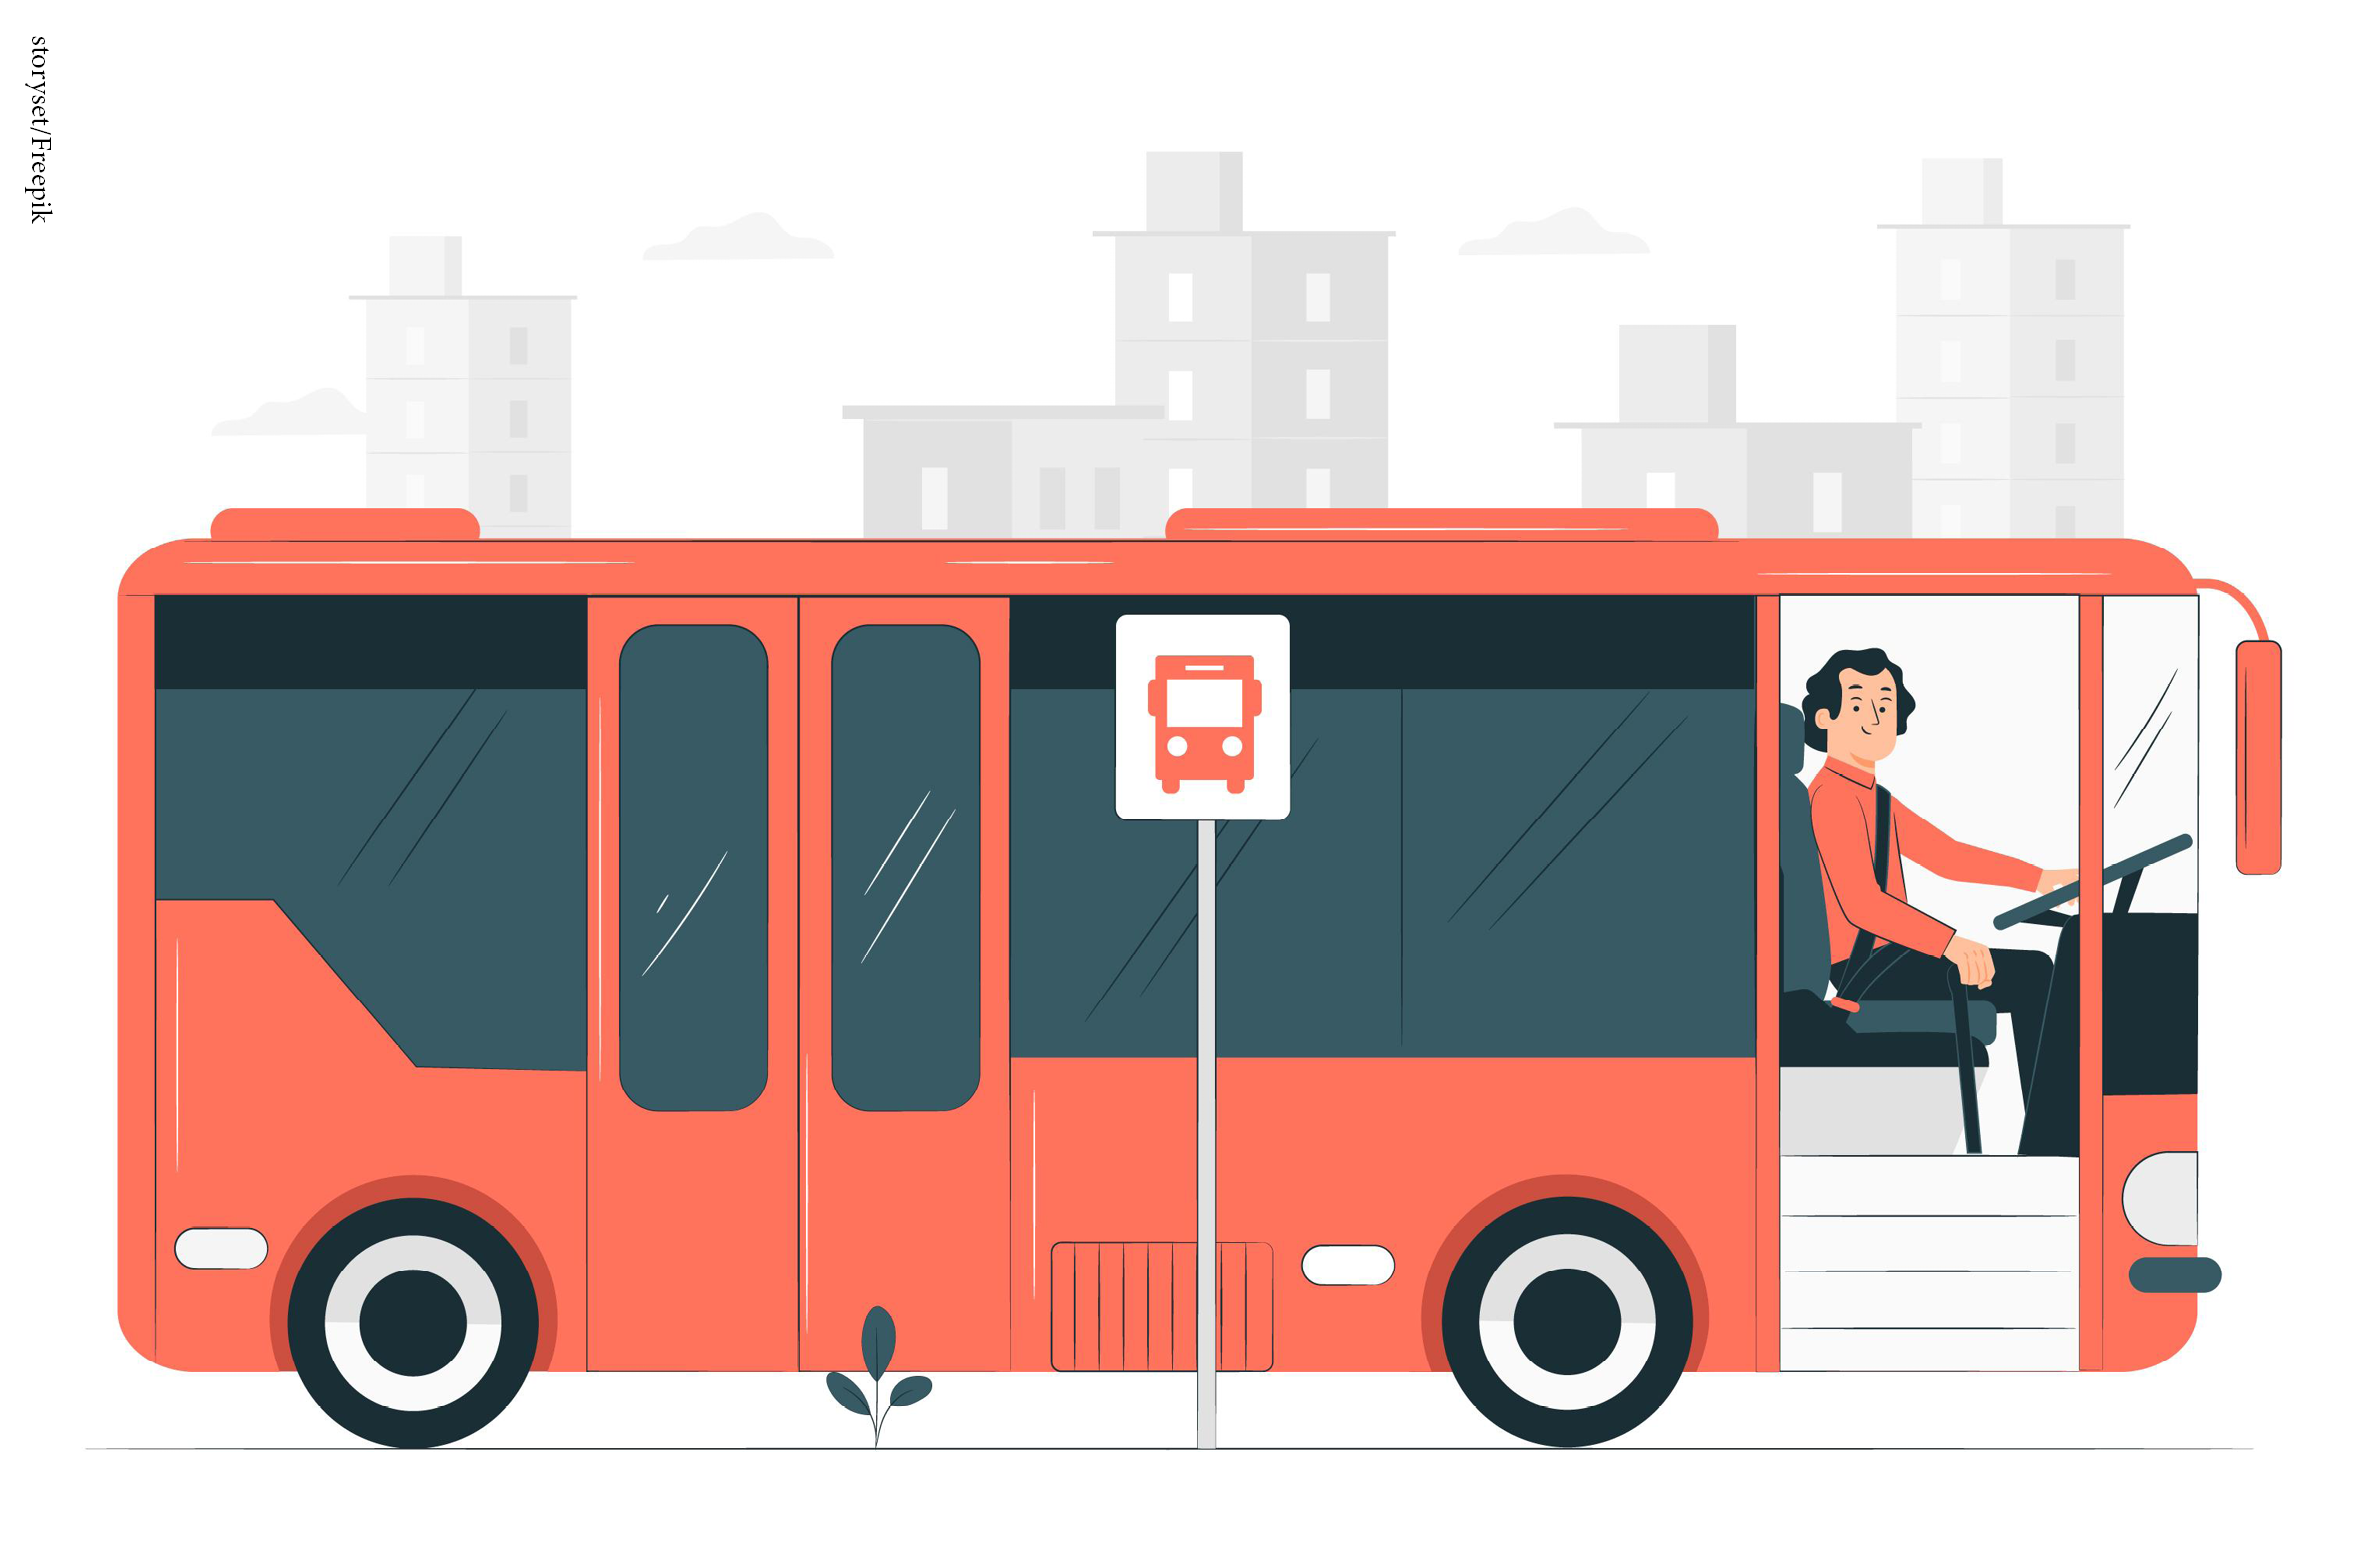
\includegraphics[width=.3\textwidth]{./media/SAEB_1ANO_MAT_FIGURA138.png}
\end{figure}

A MASSA DESSE VEÍCULO DEVE ESTAR MAIS PRÓXIMA DE

\begin{escolha}[itemsep=0pt]
\item 10 QUILOGRAMAS.

\item 5.000 QUILOGRAMAS.

\item 900 QUILOGRAMAS.

\item 50 QUILOGRAMAS.
\end{escolha}


\num{7} OBSERVE OS RELÓGIOS.

\begin{figure}[htpb!]
\centering
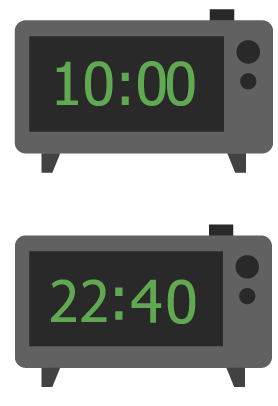
\includegraphics[width=.3\textwidth]{./media/SAEB_1ANO_MAT_FIGURA139.png}
\end{figure}

QUANTO TEMPO SE PASSOU ENTRE O HORÁRIO MARCADO PELO DA ESQUERDA E O HORÁRIO MARCADO PELO DA DIREITA?

\begin{escolha}[itemsep=0pt]
\item 10 HORAS.

\item 10 HORAS E 40 MINUTOS.

\item 12 HORAS.

\item 12 HORAS E 40 MINUTOS.
\end{escolha}

\num{8} UM JOGO DE FUTEBOL TEM 90 MINUTOS. ESSE TEMPO TAMBÉM PODE SER
REPRESENTADO POR

\begin{escolha}[itemsep=0pt]
\item 1 HORA.

\item 1 HORA E 20 MINUTOS.

\item 1 HORA E 30 MINUTOS.

\item 1 HORA E 40 MINUTOS.
\end{escolha}


\num{9} QUAL DESTES ANIMAIS APARECE EM UMA CÉDULA DE REAL?

\begin{escolha}[itemsep=0pt]
\item ARARA-VERMELHA.

\item JACARÉ-DO-PANTANAL.

\item LEÃO.

\item LEOPARDO.
\end{escolha}

\num{10} OBSERVE O ANIMAL REPRESENTADO A SEGUIR.

\begin{figure}[htpb!]
\centering
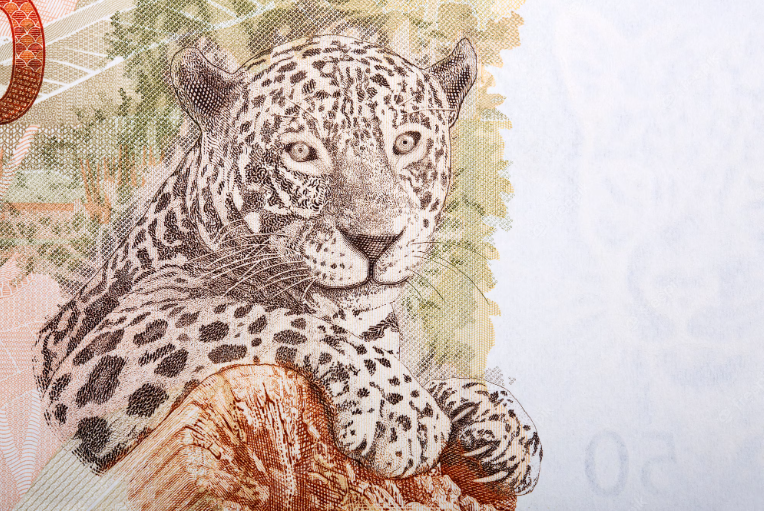
\includegraphics[width=.7\textwidth]{./media/SAEB_1ANO_MAT_FIGURA140.png}
\end{figure}

ESSE ANIMAL APARECE ESTAMPADO NAS CÉDULAS DE

\begin{multicols}{2}
\begin{escolha}[itemsep=0pt]
\item 5 REAIS.

\item 10 REAIS.

\item 20 REAIS.

\item 50 REAIS.
\end{escolha}
\end{multicols}


\num{11} OBSERVE ESTES ANIMAIS.

\begin{figure}[htpb!]
\includegraphics[width=.3\textwidth]{./media/animal1.jpg}
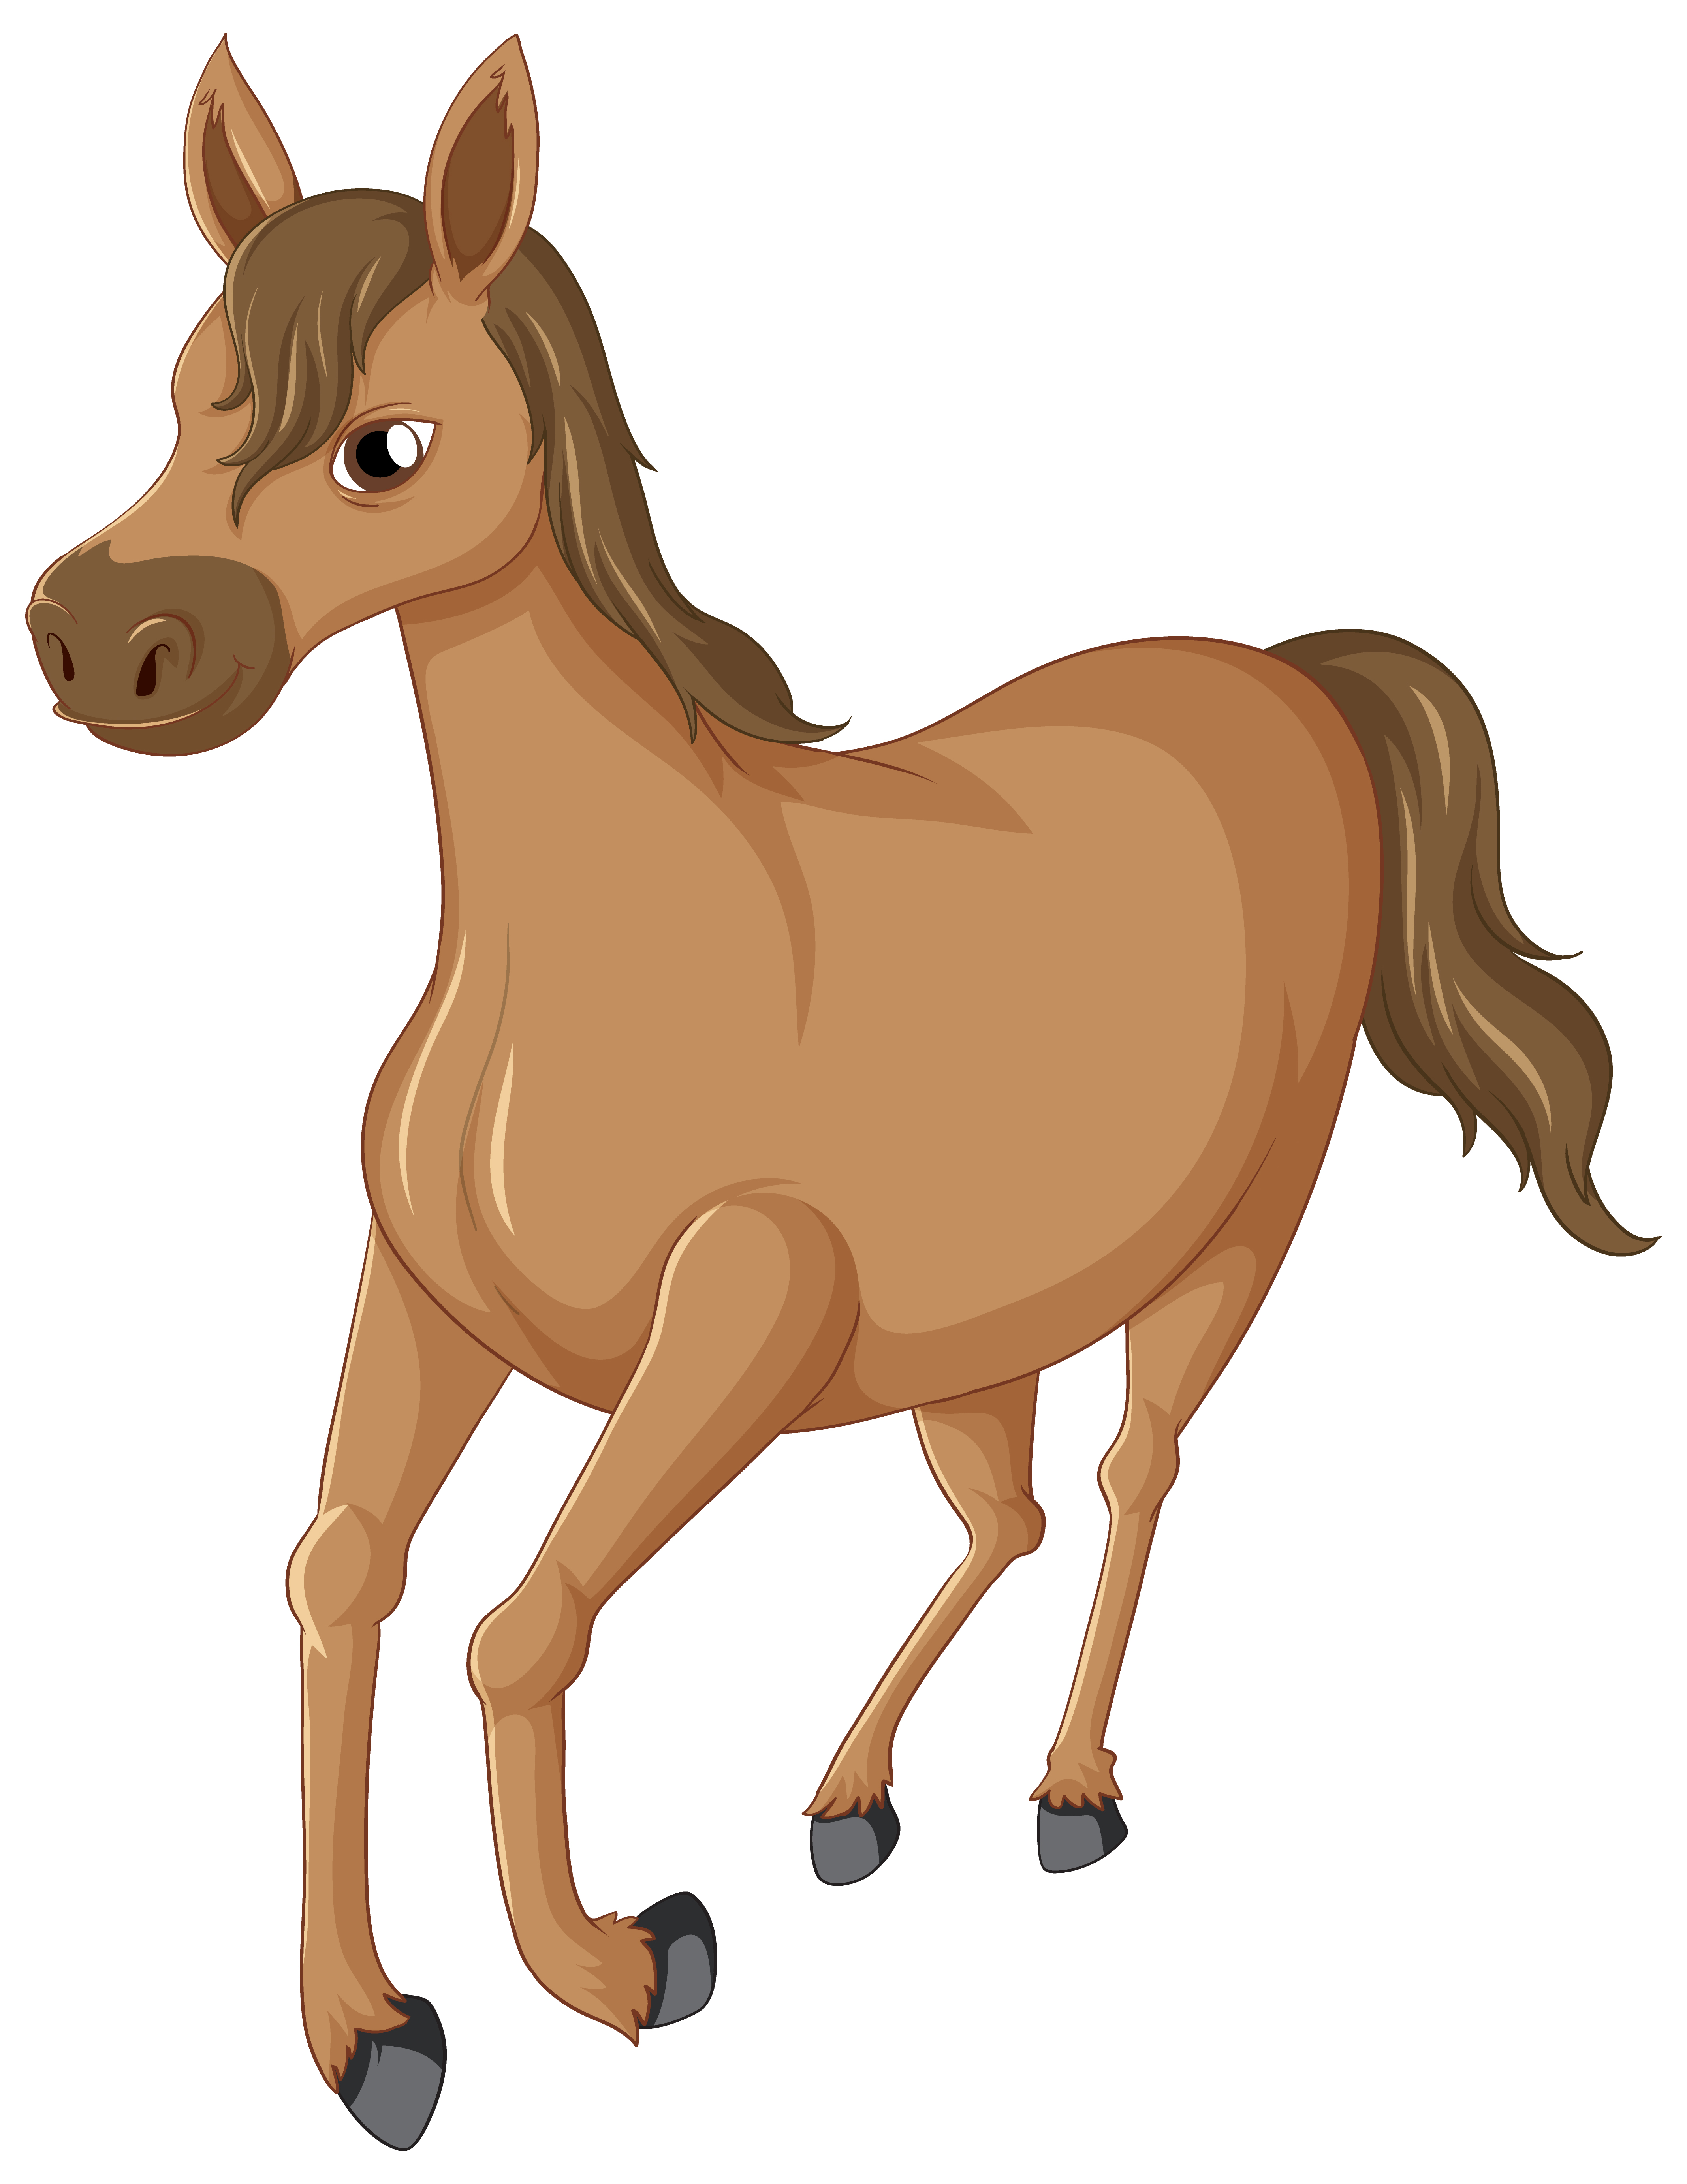
\includegraphics[width=.2\textwidth]{./media/animal2.jpg}
\includegraphics[width=.2\textwidth]{./media/animal3.jpg}

\includegraphics[width=.2\textwidth]{./media/animal4.png}
\end{figure}
 
É POSSÍVEL VOAR PARA

\begin{escolha}[itemsep=0pt]
\item A BALEIA.

\item O CAVALO.

\item O MORCEGO.

\item O TAMANDUÁ.
\end{escolha}

\num{12} AO JOGAR DOIS DADOS AO MESMO TEMPO, MARCOS SOMA O VALOR OBTIDO EM UM DADO COM O VALOR OBTIDO NO OUTRO DADO.
COM ISSO, É IMPOSSÍVEL QUE MARCOS OBTENHA A SOMATÓRIA DE

\begin{multicols}{4}
\begin{escolha}[itemsep=0pt]
\item 12.

\item 10.

\item 5.

\item 1.
\end{escolha}
\end{multicols}

\num{13} O JOGO DE CARA OU COROA É AQUELE EM QUE SE JOGA PARA O ALTO UMA MOEDA
PARA SE ANALISAR QUE LADO CAI VOLTADO PARA CIMA. UM LADO DA MOEDA É CHAMADO DE
CARA, E O OUTRO É CHAMADO DE COROA. PAULO VAI JOGAR UMA MOEDA 5 VEZES. NAS DUAS
PRIMEIRAS VEZES, A MOEDA CAIU DO LADO CARA. ENTÃO É IMPOSSÍVEL QUE SAIA O LADO
COROA

\begin{escolha}[itemsep=0pt]
\item 5 VEZES.

\item 3 VEZES.

\item 2 VEZES.

\item 1 VEZ.
\end{escolha}

\num{14} EM UMA FAMÍLIA, ALGUNS TIOS COMEÇARAM A PERGUNTAR DE QUAL COMIDA CADA
PESSOA GOSTAVA PARA PLANEJAREM O ANIVERSÁRIO DA AVÓ. OBSERVE, NO GRÁFICO A SEGUIR,
O RESULTADO DA PESQUISA.

\begin{figure}[htpb!]
\centering
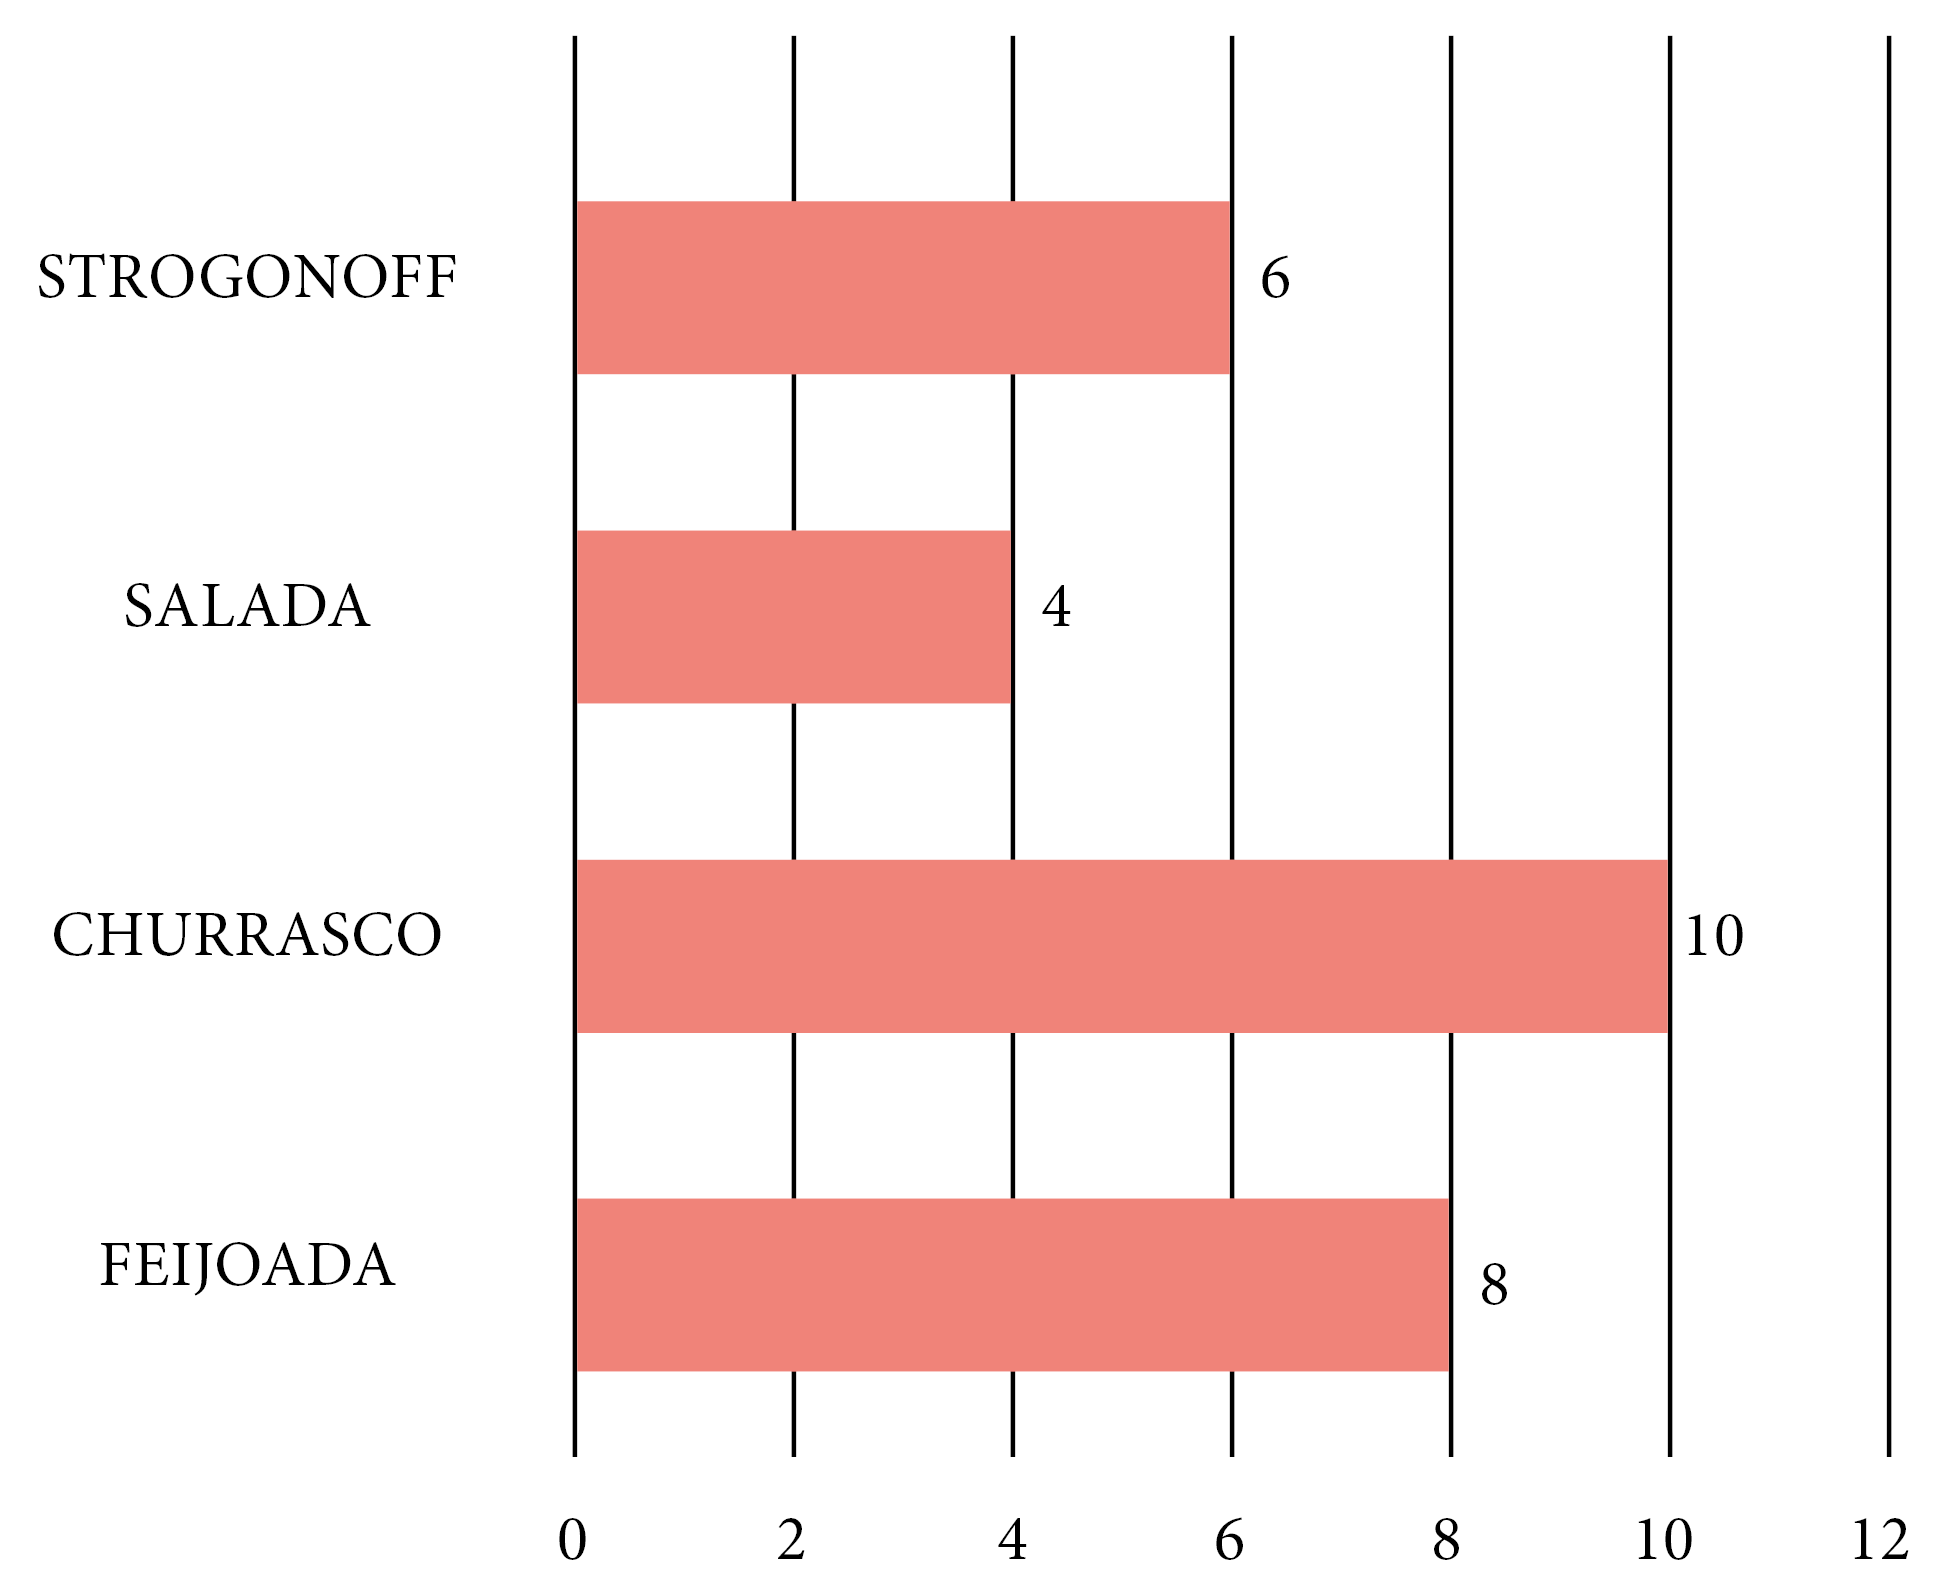
\includegraphics[width=\textwidth]{./media/SAEB_1ANO_MAT_FIGURA141.png}
\end{figure}

SE CADA UNIDADE NO GRÁFICO REPRESENTA UMA PESSOA QUE ESCOLHEU DETERMINADA COMIDA,
A DIFERENÇA ENTRE O NÚMERO DE PESSOAS QUE ESCOLHEU A MAIS VOTADA E O NÚMERO DE
PESSOAS QUE ESCOLHEU A MENOS VOTADA É

\begin{escolha}[itemsep=0pt]
\item 2.

\item 4.

\item 6.

\item 8.
\end{escolha}


\num{15} EM UMA LISTA DE MATERIAIS ESCOLARES, ENCONTRAMOS OS ITENS A SEGUIR.

% \begin{figure}[htpb!]
% \centering
% 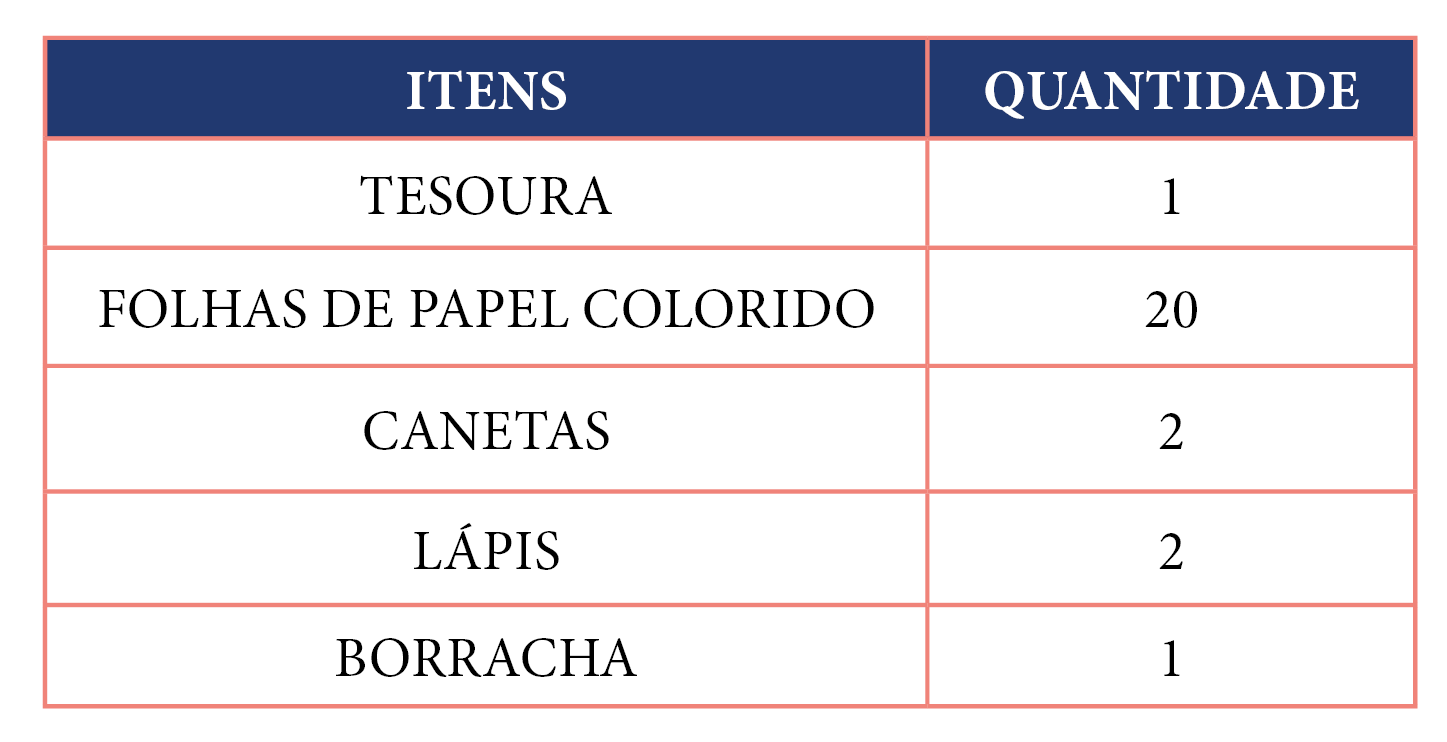
\includegraphics[width=.8\textwidth]{./media/SAEB_1ANO_MAT_FIGURA142.png}
% \end{figure}

\begin{table}[!ht]
    \centering
    \begin{tabular}{|l|l|}
    \hline
        \textbf{ITEM} & \textbf{QUANTIDADE} \\ \hline
        TESOURA & 1 \\ \hline
        FOLHA DE PAPEL COLORIDO & 20 \\ \hline
        CANETA & 2 \\ \hline
        LÁPIS & 2 \\ \hline
        BORRACHA & 1 \\ \hline
    \end{tabular}
\end{table}

QUANTOS ITENS DIFERENTES HÁ NESSA LISTA?

\begin{escolha}[itemsep=0pt]
\item 5.

\item 6.

\item 20.

\item 26.
\end{escolha}